%%%%% DOCUMENT CLASS
\documentclass[12pt]{article}

%%%%% IMPORTING PACKAGES
\usepackage{geometry} % page format
\usepackage{setspace} % page format
\usepackage{amsmath, amsthm, amssymb} % math stuff
\usepackage{mathtools} % math stuff
\usepackage{mathrsfs} % math stuff
\usepackage{empheq} % math stuff
\usepackage{cancel} % math stuff
\usepackage{tikz} % for making figures
\usepackage{graphicx} % for figures
\usepackage{placeins} % for figure placement
\usepackage{caption, subcaption} % for figures
\usepackage{enumitem} % for lists
\usepackage{matlab-prettifier} % for MATLAB code
\usepackage{verbatim} % for pasting .txt files
\usepackage{array} % table stuff
\usepackage{threeparttable} % table stuff
\usepackage{tabularx} % table stuff
\usepackage{multirow} % table stuff
\usepackage{colortbl} % table stuff
\usepackage{booktabs} % table stuff
\usepackage{pdfpages} % for importing pdfs
\usepackage{hyperref} % for hyperlinks
\usepackage{titletoc} % for TOC
\usepackage[table,dvipsnames]{xcolor} % for text coloring
\usepackage[backend=biber,sorting=none,style=numeric-comp]{biblatex} % for references
\usepackage{lipsum} % for filler
\usepackage{comment} % for comments

%%%%% CONFIGURING PACKAGE SETTINGS
\geometry{letterpaper,left=1in,top=1in,right=1in,bottom=1in}
\onehalfspacing % as per writing guidelines
\graphicspath{ {./Figures/} }
\allowdisplaybreaks[1]
\hypersetup{colorlinks=true, linkcolor=red, filecolor=magenta, urlcolor=black, citecolor=blue}
\addbibresource{bib.bib}

%%%%% CREATING CUSTOM COMMANDS
\newcommand{\mainmatter}{\clearpage\setcounter{page}{1}\pagenumbering{arabic}}
\newcommand{\appendixpagenumbering}{\clearpage\pagenumbering{arabic}\renewcommand{\thepage}{A-\arabic{page}}}
\newcommand\innercontentsname[1]{%
Contents for section~\ref{#1}}
\newcolumntype{P}[1]{>{\centering\arraybackslash}p{#1}}
\newcolumntype{M}[1]{>{\centering\arraybackslash}m{#1}}
\newcolumntype{R}[1]{>{\raggedleft\arraybackslash}m{#1}}
\renewcommand\tabularxcolumn[1]{m{#1}}

% whatever math operators we need
\DeclareMathOperator{\sgn}{sgn}
\DeclareMathOperator{\acos}{acos}
\DeclareMathOperator{\atantwo}{atan2}
\DeclareMathOperator{\spec}{Spec}

%%%%% DOCUMENT
\begin{document}

%%%%% TITLE PAGE
\begin{titlepage}
\begin{center}
    \vspace*{\fill}
    {\Huge Engineering Collective Intelligence}\\
    {\large MAE 6870 Homework 2}

    \vspace{4\baselineskip}
    Daniel Whitman\\
    % Engineering Collective Intelligence (MAE 6870)\\
    10/26/2026
\end{center}

% \vspace{4\baselineskip}
% \noindent \textbf{ABSTRACT:}
% \noindent 

\vspace*{\fill}
\end{titlepage}

%%%%% ABSTRACT PAGE
% \clearpage
% \pagenumbering{gobble}
% \section*{ABSTRACT}
% \noindent Words

%%%%% ACTUAL REPORT
\mainmatter
\section*{AI STATEMENT}
I did not use AI for this assignment outside of the AI summary that Google provides when searching something up, which was all related to how to implement something in Python (e.g., how to plot a grid in Python, etc.).

\section*{PROBLEM SOLUTIONS}\label{sec:problems}
\subsection*{1.}
\textbf{Proximity graph and sensing neighborhoods.}
Construct the true temperature field and visualize each robot's sensing neighborhood. Draw the communication graph, report each robot's degree, and identify any robots whose removal would disconnect the graph. Construct $W$ and verify that the graph is connected and $W$ is doubly stochastic. How many robots measure each cell? Does the team cover the entire floor? In code, implement a measurement function following (\ref{eqn:measurement}) which takes $\theta$ and $\sigma_i$ as arguments and outputs a measurement $y_i$ of $\theta$.

\vspace{\baselineskip}
\noindent\textbf{ANSWER:}

The true temperature field was constructed and is visualized in Figure \ref{fig:true_temperature_graph_network}, as well as the connected communication graph. As seen in this Figure, the field is completely covered by all robots, and there are \textit{no} cells that are not being measured. However, there are some cells that are being measured by multiple robots (e.g., cell (3,3) being measured by robots 1, 2, and 7) and some cells that are being measured by only one robot (e.g., cell (0,9) being measured by robot 3). If we display the number of robots measuring each cell as a matrix (with row and column corresponding to row and column number in the grid), we have
\begin{align*}
    |\mathcal S_{rc}|&=\begin{pmatrix}
        1 & 1 & 1 & 1 & 2 & 1 & 1 & 1 & 1 & 1\\
        1 & 1 & 1 & 2 & 3 & 2 & 1 & 2 & 2 & 2\\
        2 & 2 & 3 & 2 & 3 & 2 & 3 & 2 & 2 & 2\\
        2 & 3 & 3 & 3 & 1 & 3 & 3 & 3 & 2 & 2\\
        2 & 3 & 3 & 2 & 2 & 2 & 3 & 3 & 2 & 1\\
        1 & 2 & 3 & 3 & 3 & 2 & 3 & 3 & 2 & 1\\
        1 & 2 & 3 & 3 & 3 & 3 & 3 & 2 & 2 & 2\\
        2 & 2 & 2 & 3 & 3 & 3 & 2 & 2 & 2 & 2\\
        2 & 2 & 2 & 1 & 2 & 2 & 2 & 1 & 1 & 1\\
        1 & 1 & 1 & 1 & 2 & 2 & 2 & 1 & 1 & 1
    \end{pmatrix}.
\end{align*}
Note: this matrix will seem ``upside-down'' compared to visually what appears in Figure \ref{fig:true_temperature_graph_network} as the matrix is indexed from the top-left corner and the grid is indexed from the bottom-left corner.

\begin{figure}[htb]
    \centering
    \begin{subfigure}[t]{0.45\textwidth}
        \centering
        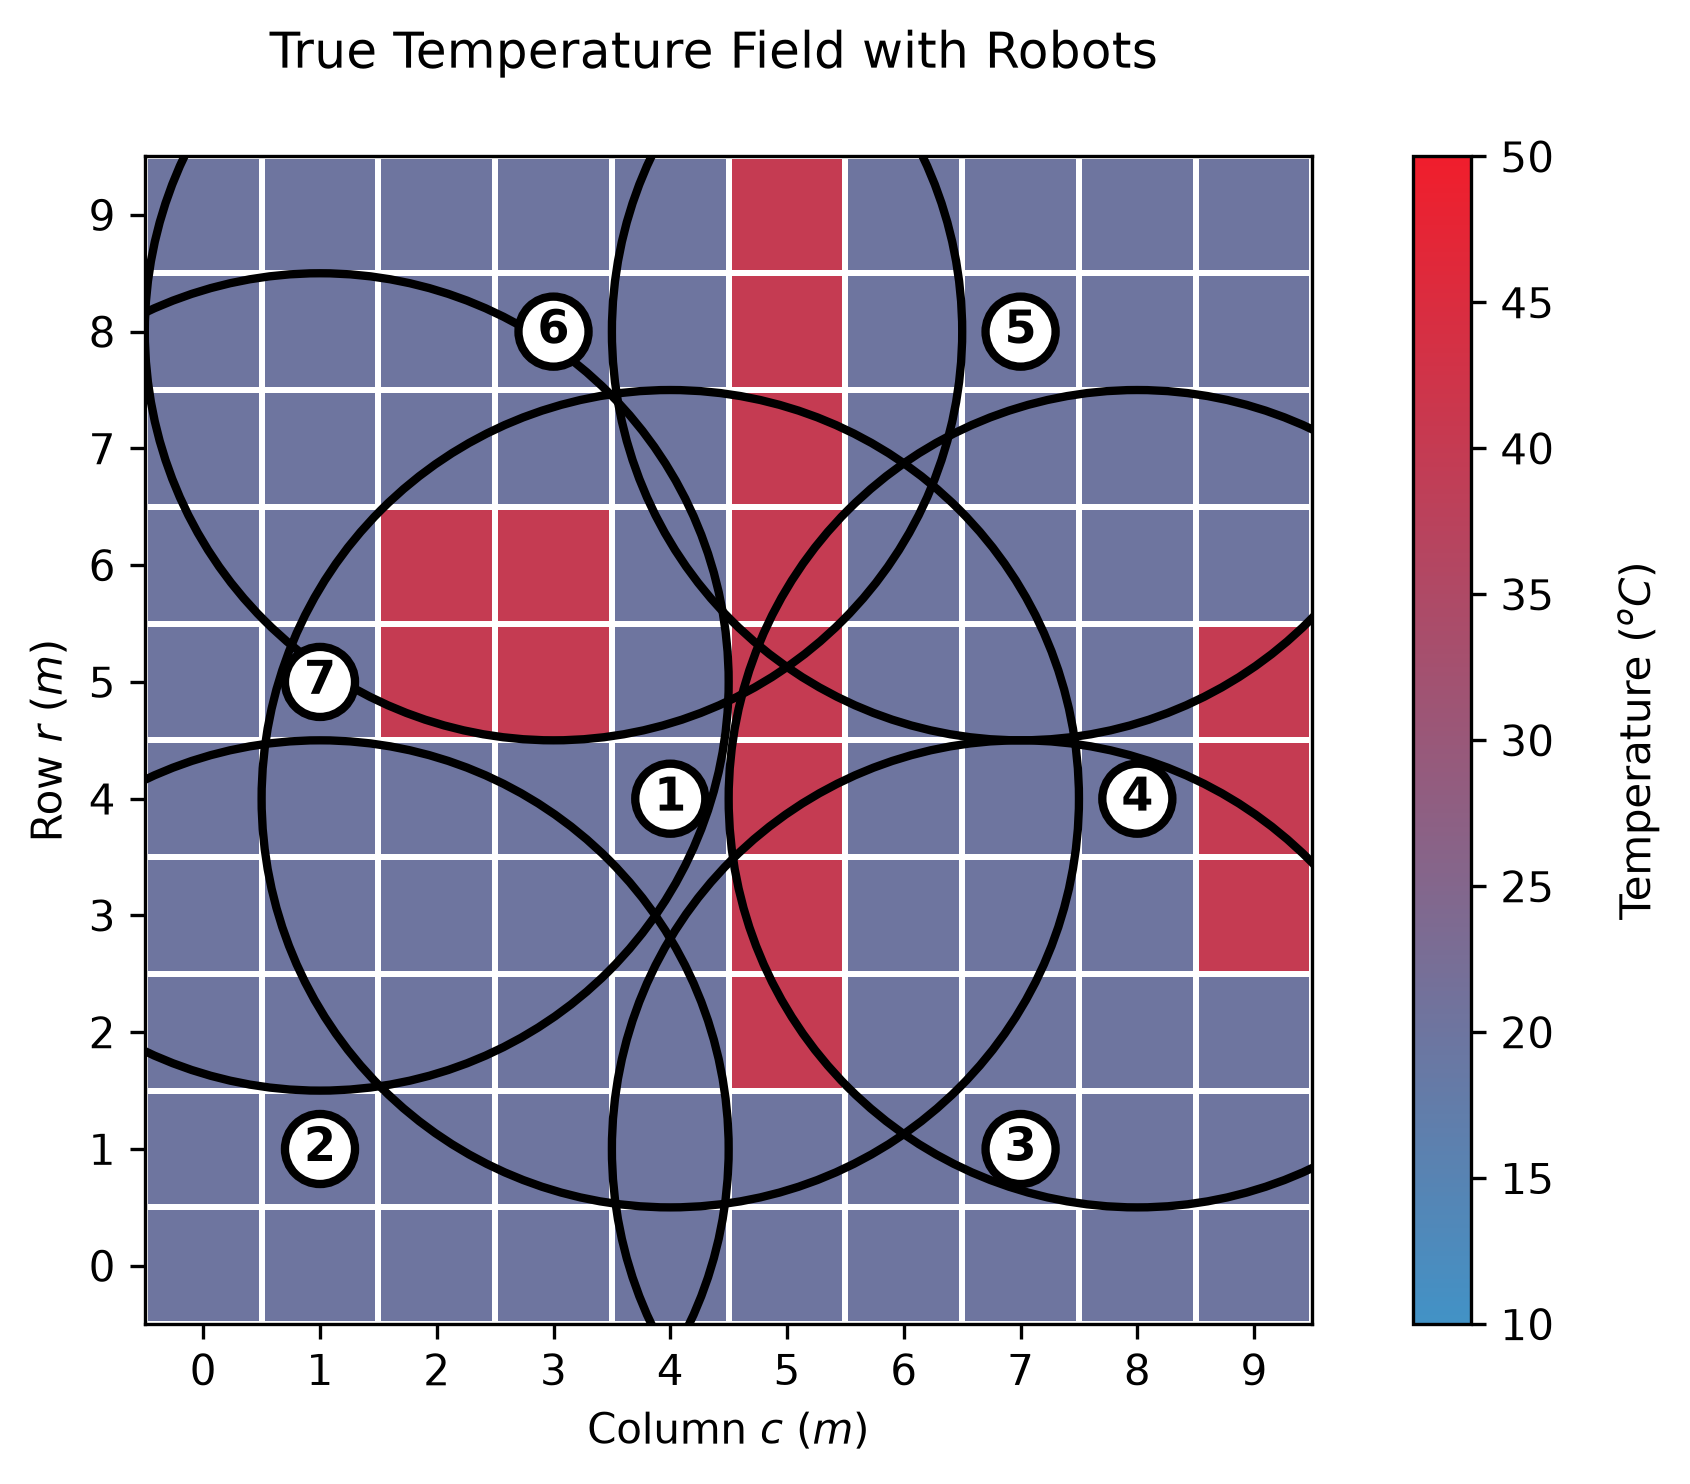
\includegraphics[width=\textwidth]{Figures/true_temperature.png}
        \captionsetup{justification=centering}
        \caption{True temperature field overlaid with the robots (numbered tokens) and their respective sensing neighborhoods (circles).}
        % \label{fig:}
    \end{subfigure}\hfill
    \begin{subfigure}[t]{0.45\textwidth}
        \centering
        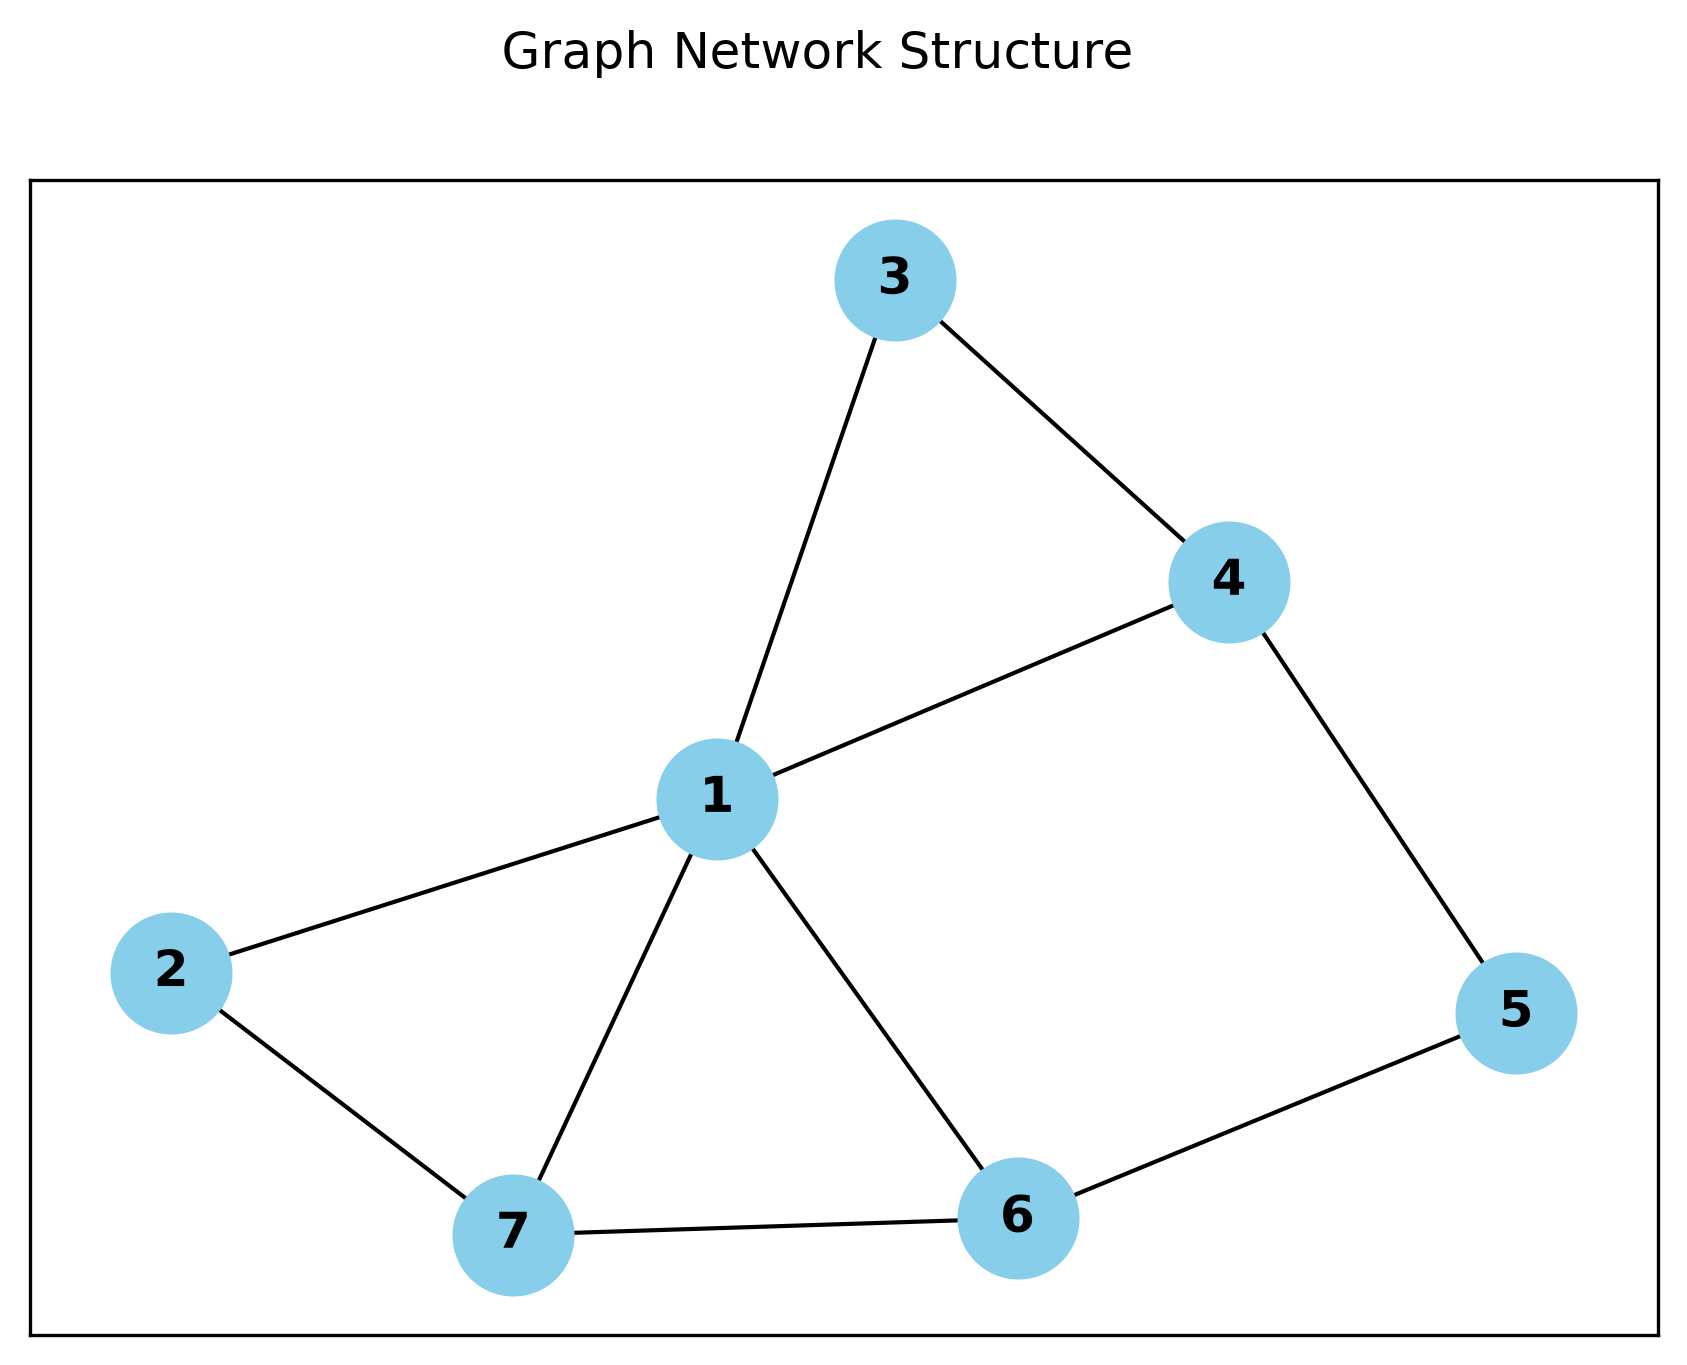
\includegraphics[width=\textwidth]{Figures/graph_network.png}
        \captionsetup{justification=centering}
        \caption{Graph network structure displaying connections between the robots.}
        % \label{fig:}
    \end{subfigure}
    \captionsetup{justification=centering}
    \caption{}
    \label{fig:true_temperature_graph_network}
\end{figure}

As for the network structure in Figure \ref{fig:true_temperature_graph_network}, there is no single robot that can be removed that would cause the graph to be disconnected. While robot 1 is clearly more connected than the others, if removed, the others would form a ``line'' network and remain connected. To disconnect the graph, 2 or more robots would need to be removed (such as removing both robots 1 \textit{and} 5). Additionally, from this network, we can see that each robot's in-degree is, in order:
\begin{align*}
    \Aboxed{\text{in-degree}&=\{5,2,2,3,2,3,3\}}
\end{align*}

For this network, the consensus weight matrix $W$ was constructed following the metropolis weight formulation:
\begin{align}\label{eqn:metropolis}
    w_{ij}&=\begin{cases}
        \frac{1}{1+\max\{d_i,d_j\}}& j\in\mathcal N_i\\
        1-\sum_{\ell\in\mathcal N_i}w_{i\ell} & j=i\\
        0 & \text{otherwise}.
    \end{cases}
\end{align}

With this formulation, the robot in-degrees, and the connections given in Figure \ref{fig:true_temperature_graph_network}, the weight matrix $W$ was found to be
\begin{align}\label{eqn:W}
    W&=\begin{pmatrix}
        \frac16 & \frac16 & \frac16 & \frac16 & 0 & \frac16 & \frac16\\
        \frac16 & \frac7{12} & 0 & 0 & 0 & 0 & \frac14\\
        \frac16 & 0 & \frac7{12} & \frac14 & 0 & 0 & 0\\
        \frac16 & 0 & \frac14 & \frac13 & \frac14 & 0 & 0\\
        0 & 0 & 0 & \frac14 & \frac12 & \frac14 & 0\\
        \frac16 & 0 & 0 & 0 & \frac14 & \frac13 & \frac14\\
        \frac16 & \frac14 & 0 & 0 & 0 & \frac14 & \frac13
    \end{pmatrix}.
\end{align}

It is easy to confirm that this matrix is indeed doubly-stochastic, which means that all of its rows \textit{and} all of its columns sum to 1. We can see this simply by multiplying by the vector $\mathbf1$ for both $W$ (shows row-stochasticity) and $W^T$ (shows column-stochasticity):
\begin{align*}
    W\mathbf1&=\begin{pmatrix}
        1\\1\\1\\1\\1\\1\\1
    \end{pmatrix}, & W^T\mathbf1&=\begin{pmatrix}
        1\\1\\1\\1\\1\\1\\1
    \end{pmatrix}.
\end{align*}

To verify that the graph $W$ is indeed connected, we can look at its eigenvalues. As the communication protocol is \textit{discrete}, we should expect to see a \textit{unique} eigenvalue of 1 (the consensus mode) with all others $|\lambda_i|<1,\ i\neq1$. When computing the spectrum of $W$, the eigenvalues are (computed with \texttt{Python}):
\begin{align*}
    \lambda_i\in\spec(W)=\{1.0,\ 0.7749,\ 0.6512,\ 0.3735,\ 0.1250,\ 0.02670,\ -0.1181\}.
\end{align*}
As seen, this matches the expected result where only a single eigenvalue is equal to 1, showing there is only one consensus mode and that the graph is strongly connected.

\clearpage
\subsection*{2.}
\textbf{Temperature mapping.}
Consider one cell measurement by $n_{rc}=|\mathcal S_{rc}|>0$ robots. Treat its temperature $\theta_{rc}\in\mathbb R$ as an unknown scalar.

\begin{enumerate}[label=(\alph*)]
    \item Write the Gaussian likelihood and derive the maximum-likelihood estimate $\hat\theta_{rc}^w$ when the variances $\sigma_i^2$ are known. Show that equal variances give the ordinary mean of the available measurements. We will define $\hat\theta_{rc}^u$ to be this unweighted mean. \textit{Hint, we did a version of this calculation in class!}
    \item Compute the bias and variance of the weighted estimate $\hat\theta_{rc}^w$ and the unweighted estimate $\hat\theta_{rc}^u$ under the measurement model (\ref{eqn:measurement}). Which has smaller expected squared error when the variances differ? Justify your answer. What happens if only one robot measures the cell? \textit{Hint: write each estimate as $\sum_{i\in\mathcal S_{rc}}\beta_iy_{rc}^{(i)}$, identify its coefficients, and apply (\ref{eqn:gaussian_bv}). To compare the resulting variances, you may use the following inequality, which is a consequence of Cauchy-Schwarz}
    \begin{align}\label{eqn:varcomp}
        \left(\sum_{i\in\mathcal S_{rc}}\sigma_i^2\right)\left(\sum_{i\in\mathcal S_{rc}}\sigma_i^{-2}\right)\geq n_{rc}^2.
    \end{align}
\end{enumerate}

\noindent\textbf{ANSWER:}
\begin{enumerate}[label=(\alph*)]
    \item A Gaussian likelihood for robot $i$'s measurement $\theta_{irc}$ of the true temperature $\theta_{rc}$ is given as
    \begin{align*}
        \mathscr L_i(\theta_{rc},\theta_{irc})&=\frac{1}{\sqrt{2\pi\sigma_i^2}}\exp\left(\frac{-(\theta_{irc}-\theta_{rc})^2}{2\sigma_i^2}\right),
    \end{align*}
    so the total maximum-likelihood function given all robot measurements is
    \begin{align*}
        \mathscr L(\theta_{rc},\theta_{irc})&=\prod_{i=1}^{n_{rc}}\frac{1}{\sqrt{2\pi\sigma_i^2}}\exp\left(\frac{-(\theta_{irc}-\theta_{rc})^2}{2\sigma_i^2}\right).
    \end{align*}

    To find the maximum-likelihood estimate $\hat\theta_{rc}^w$, we can convert this expression into the \textit{log-likelihood} to simplify the mathematics as
    \begin{align*}
        \ell(\theta_{rc},\theta_{irc})&=\log(\mathscr L(\theta_{rc},\theta_{irc}))\\
        &=\log\left(\prod_{i=1}^{n_{rc}}\frac{1}{\sqrt{2\pi\sigma_i^2}}\exp\left(\frac{-(\theta_{irc}-\theta_{rc})^2}{2\sigma_i^2}\right)\right)\\
        &=-\frac12\sum_{i=1}^{n_{rc}}\log(2\pi\sigma_i^2)+\sum_{i=1}^{n_{rc}}\frac{-(\theta_{irc}-\theta_{rc})^2}{2\sigma_i^2}.
    \end{align*}

    To then find the maximum-likelihood estimate, we differentiate the log-likelihood expression and find its extrema. So,
    \begin{align}
        \ell'(\theta_{rc},\theta_{irc})[\hat\theta_{rc}^w]&=0\nonumber\\
        \frac{d}{d\theta_{rc}}\left.\left(-\frac12\sum_{i=1}^{n_{rc}}\log(2\pi\sigma_i^2)+\sum_{i=1}^{n_{rc}}\frac{-(\theta_{irc}-\theta_{rc})^2}{2\sigma_i^2}\right)\right|_{\theta_{rc}=\hat\theta_{rc}^w}&=0\nonumber\\
        \sum_{i=1}^{n_{rc}}\frac{\theta_{irc}-\hat\theta_{rc}^w}{2\sigma_i^2}&=0\nonumber\\
        \sum_{i=1}^{n_{rc}}\frac{\hat\theta_{rc}^2}{\sigma_i^2}&=\sum_{i=1}^{n_{rc}}\frac{\theta_{irc}}{\sigma_i^2}\nonumber\\
        \hat\theta_{rc}^w&=\frac{\sum_{i=1}^{n_{rc}}\frac{\theta_{irc}}{\sigma_i^2}}{\sum_{i=1}^{n_{rc}}\frac{1}{\sigma_i^2}}.\label{eqn:theta_w}
    \end{align}

    In this expression, we can see that each measurement is weighted by the inverse of its variance $(1/\sigma_i^2)$, which is then normalized by the sum of \textit{all} the inverse-variances such that the sum of the normalized weights equals 1. If we now state that the variances are identical (i.e., $\sigma_i^2=\sigma^2,\ \forall i$), this expression simplifies to the unweighted mean $\hat\theta_{rc}^u$:
    \begin{align}
        \hat\theta_{rc}^u&=\frac{\sum_{i=1}^{n_{rc}}\frac{\theta_{irc}}{\sigma^2}}{\sum_{i=1}^{n_{rc}}\frac{1}{\sigma^2}}\nonumber\\
        &=\frac{\frac{1}{\sigma^2}\sum_{i=1}^{n_{rc}}\theta_{irc}}{\frac{1}{\sigma^2}\sum_{i=1}^{n_{rc}}1}\nonumber\\
        \hat\theta_{rc}^u&=\frac{1}{n_{rc}}\sum_{i=1}^{n_{rc}}\theta_{irc}.\label{eqn:theta_u}
    \end{align}

    \item We can now compute the bias and the variance for both the weighted estimate (\ref{eqn:theta_w}) and the unweighted estimate (\ref{eqn:theta_u}) for comparison. The bias for a given expression is given as
    \begin{align}\label{eqn:bias}
        \text{Bias}(\hat\theta)&=\mathbb E(\hat\theta)-\theta,
    \end{align}
    and the variance is given as
    \begin{align}\label{eqn:variance}
        \text{Var}(\hat\theta)&=\mathbb E(\hat\theta^2)-(\mathbb E(\hat\theta))^2.
    \end{align}

    For our Gaussian measurement given as
    \begin{align}\label{eqn:measurement}
        y_{rc}^{(i)}&=\theta_{rc}+\varepsilon_{rc}^{(i)}, & \varepsilon_{rc}^{(i)}\sim\mathcal N(0,\sigma_i^2),
    \end{align}
    we can equivalently calculate the bias and variance as
    \begin{align}\label{eqn:gaussian_bv}
        \text{Bias}(\hat\theta)&=-\theta+\sum_{i=1}^n\beta_i\mathbb E(\theta_i) & \text{Var}(\hat\theta)&=\sum_{i=1}^n\beta_i^2\text{Var}(\theta_i),
    \end{align}
    where $\beta_i$ are some fixed coefficients. Now, using (\ref{eqn:gaussian_bv}), we can find the bias and variance for both the weighted estimate (\ref{eqn:theta_w}) and unweighted estimate (\ref{eqn:theta_u}). First, let us begin with the bias for the weighted estimate:
    \begin{align*}
        \text{Bias}(\hat\theta_{rc}^w)&=-\theta_{rc}+\mathbb E(\hat\theta_{rc}^w)\\
        &=-\theta_{rc}+\mathbb E\left(\frac{\sum_{i=1}^{n_{rc}}\frac{\theta_{irc}}{\sigma_i^2}}{\sum_{i=1}^{n_{rc}}\frac{1}{\sigma_i^2}}\right).
    \end{align*}

    For simplification, let us define
    \begin{align}\label{eqn:omega}
        \sum_{i=1}^{n_{rc}}\frac{1}{\sigma_i^2}&=\Omega
    \end{align}
    such that our weighted bias then becomes
    \begin{align*}
        \text{Bias}(\hat\theta_{rc}^w)&=-\theta_{rc}+\mathbb E\left(\sum_{i=1}^{n_{rc}}\frac{\theta_{irc}}{\Omega\sigma_i^2}\right)\\
        &=-\theta_{rc}+\sum_{i=1}^{n_{rc}}\frac{\mathbb E(\theta_{irc})}{\Omega\sigma_i^2},
    \end{align*}
    where we can clearly see that, in the weighted case,
    \begin{align}\label{eqn:bw}
        \beta_i^w&=\frac{1}{\Omega\sigma_i^2}.
    \end{align}
    Completing the derivation of the bias, we have
    \begin{align*}
        \text{Bias}(\hat\theta_{rc}^w)&=-\theta_{rc}+\sum_{i=1}^{n_{rc}}\frac{\theta_{rc}}{\Omega\sigma_i^2}\\
        &=-\theta_{rc}+\frac{\Omega}{\Omega}\theta_{rc}\\
        \Aboxed{\text{Bias}(\hat\theta_{rc}^w)&=-\theta_{rc}+\theta_{rc}=0}.
    \end{align*}
    
    The unweighted bias is then
    \begin{align*}
        \text{Bias}(\hat\theta_{rc}^u)&=-\theta_{rc}+\mathbb E(\hat\theta_{rc}^u)\\
        &=-\theta_{rc}+\mathbb E\left(\frac{1}{n_{rc}}\sum_{i=1}^{n_{rc}}\theta_{irc}\right)\\
        &=-\theta_{rc}+\sum_{i=1}^{n_{rc}}\frac{\mathbb E(\theta_{irc})}{n_{rc}},
    \end{align*}
    where our unweighted coefficients are
    \begin{align}\label{eqn:bu}
        \beta_i^u&=\frac{1}{n_{rc}}.
    \end{align}
    Completing the derivation of the bias, we have
    \begin{align*}
        \text{Bias}(\hat\theta_{rc}^u)&=-\theta_{rc}+\sum_{i=1}^{n_{rc}}\frac{\theta_{rc}}{n_{rc}}\\
        &=-\theta_{rc}+\frac{\theta_{rc}}{n_{rc}}\sum_{i=1}^{n_{rc}}1\\
        &=-\theta_{rc}+\frac{n_{rc}}{n_{rc}}\theta_{rc}\\
        \Aboxed{\text{Bias}(\hat\theta_{rc}^u)&=-\theta_{rc}+\theta_{rc}=0}.
    \end{align*}

    Next, let us find the variance of the weighted estimate using (\ref{eqn:bw}):
    \begin{align}
        \text{Var}(\hat\theta_{rc}^w)&=\sum_{i=1}^{n_{rc}}(\beta_i^w)^2\text{Var}(\theta_{irc})\nonumber\\
        &=\sum_{i=1}^{n_{rc}}\left(\frac{1}{\Omega\sigma_i^2}\right)^2\sigma_i^2\nonumber\\
        &=\frac{1}{\Omega^2}\sum_{i=1}^{n_{rc}}\frac{1}{\sigma_i^2}\nonumber\\
        \Aboxed{\text{Var}(\hat\theta_{rc}^w)&=\frac{1}{\Omega}=\frac{1}{\sum_{i=1}^{n_{rc}}\frac{1}{\sigma_i^2}}}.\label{eqn:varw}
    \end{align}

    The variance of the unweighted estimate is then, using (\ref{eqn:bu}):
    \begin{align}
        \text{Var}(\hat\theta_{rc}^u)&=\sum_{i=1}^{n_{rc}}(\beta_i^u)^2\text{Var}(\theta_{irc})\nonumber\\
        &=\sum_{i=1}^{n_{rc}}\left(\frac{1}{n_{rc}}\right)^2\sigma_i^2\nonumber\\
        \Aboxed{\text{Var}(\hat\theta_{rc}^u)&=\frac{1}{n_{rc}^2}\sum_{i=1}^{n_{rc}}\sigma_i^2}.\label{eqn:varu}
    \end{align}

    Note, that in this case, with the MSE given as
    \begin{align}
        \text{MSE}(\hat\theta)&=\text{Var}(\hat\theta)+\text{Bias}(\hat\theta)^2,
    \end{align}
    as both the weighted and unweighted biases are 0, the MSE becomes identical to our variance. Therefore, we can compare relative MSE through the variances (\ref{eqn:varw}) and (\ref{eqn:varu}) using the inequality in (\ref{eqn:varcomp}). So,
    \begin{align*}
        \left(\sum_{i=1}^{n_{rc}}\sigma_i^2\right)\left(\sum_{i=1}^{n_{rc}}\frac{1}{\sigma_i^2}\right)&\geq n_{rc}^2\\
        \left(\frac{1}{n_{rc}^2}\sum_{i=1}^{n_{rc}}\sigma_i^2\right)(\Omega)&\geq 1\\
        \text{Var}(\hat\theta_{rc}^u)&\geq\frac{1}{\Omega}\\
        \Aboxed{\text{Var}(\hat\theta_{rc}^u)&\geq\text{Var}(\hat\theta_{rc}^u)}.
    \end{align*}

    From this, we can clearly see that when the variances differ (and as a result the MSEs differ), the \textit{unweighted} case will have a much larger error than the weighted case. Intuitively, this makes sense, because if we weight a very inaccurate measurement equally with the others (as in the unweighted case), it will impact the estimate much more detrimentally than if we scale it appropriately according to its own variance. We should scale each measurement based on how ``confident'' we are in its accuracy. However, in the case where $n_{rc}=1$ (only one robot measures a cell), (\ref{eqn:varw}) and (\ref{eqn:varu}) become:
    \begin{align*}
        \text{Var}(\hat\theta_{rc}^2)&=\frac{1}{\Omega} & \text{Var}(\hat\theta_{rc}^u)&=\frac{1}{1^2}\sum_{i=1}^1\sigma_i^2\\
        &=\frac{1}{\sum_{i=1}^1\frac{1}{\sigma_i^2}} & &=\sigma_1^2\\
        &=\frac{1}{\frac{1}{\sigma_1^2}} & &\\
        &=\sigma_1^2,
    \end{align*}
    where we can clearly see that they are equal. So, weighting the measurements \textit{only} benefits if a cell is being measured by more than one robot, else we can just take the singular measurement as the estimate itself.
\end{enumerate}

\clearpage
\subsection*{3.}
\textbf{Fuse one sensing round over the graph with identical sensors.}
Based on the sensor fusion formula we derived in class and in Part 2, to synchronize a heat map estimate across the graph, each robot must estimate two scalar states per cell: a weighted sum of the measurements of all robots, $a_{rc}^{(i)}=\sum_{i=1}^n\alpha_iy_{rc}^{(i)}$ and the sensor coefficient sum $b_{rc}^{(i)}=\sum_{i=1}^n\alpha_i$, with sensor coefficients defined as
\begin{align*}
    \alpha_i&=1\ \text{for unweighted fusion,} & \alpha_i=\sigma_i^{-2}\ \text{for uncertainty-weighted fusion.}
\end{align*}

At the initial step of the fusion algorithm, we will assume
\begin{align}\label{eqn:init}
    \left(a_{rc}^{(i)}(0),b_{rc}^{(i)}(0)\right)&=\begin{cases}
        (\alpha_iy_{rc}^{(i)},\alpha_i), & i\in\mathcal S_{rc},\\
        (0,0), & i\notin\mathcal S_{rc}.
    \end{cases}
\end{align}

To fuse the measurement, each robot will run tow averaging consensus updates in parallel,
\begin{align}\label{eqn:consensus}
    a_{rc}^{(i)}(k+1)&=\sum_{j=1}^7w_{ij}a_{rc}^{(i)}(k), & b_{rc}^{(i)}(k+1)&=\sum_{j=1}^7w_{ij}b_{rc}^{(j)}(k).
\end{align}
where $k$ is the index associated with the consensus round. Whenever $b_{rc}^{(i)}(k)>0$, robot $i$ forms the temperature estimate
\begin{align}\label{eqn:temp_estimate}
    x_{rc}^{(i)}(k)&=\frac{a_{rc}^{(i)}(k)}{b_{rc}^{(i)}(k)}
\end{align}
Otherwise its estimate of that cell is unknown.

\begin{enumerate}[label=(\alph*)]
    \item Write down the limits of $a_{rc}^{(i)}$ and $b_{rc}^{(i)}$ as $k\to\infty$, assuming the communication graph is connected. Does their ratio converge to the appropriate estimate from Part 2?
    \item Implement (\ref{eqn:init})--(\ref{eqn:temp_estimate}) in code assuming $\sigma_i^2=25\ (^oC)^2$ for all $i=1,\dots,7$, corresponding to standard deviations of $5^oC$. Let each robot take one measurement, and run $K=100$ consensus round to fuse the estimate. At the final time step, compare and report the maximum absolute difference from the corresponding centralized formula across all robots and observed cells.
    \item For cell $(5,5)$, plot all seven estimates $x_{55}^{(i)}(k)$ and the centralized estimate as function of $k$. Leave an estimate undefined until its denominator is positive. How can a robot estimate temperatures beyond its own sensing range?
    \item Discuss the observed effects of cooperation on \textit{convergence} (i.e., how much of the total map area is each robot able to construct with and without cooperation?) and on \textit{accuracy} where measurements overlap (i.e., what happens to the estimate uncertainty when more than one robot can measure a particular cell?). To compare accuracy numerically, evaluate the local and fused estimates on the set $\mathcal V^{(1)}$ (i.e. cells visible to robot 1) and compare the expected MSE and per-cell variances over this same set for the estimate of $a_{rc}$.
\end{enumerate}

\noindent\textbf{ANSWER:}
\begin{enumerate}[label=(\alph*)]
    \item Let us consider the limits of $a_{rc}^{(i)}$ and $b_{rc}^{(i)}$ as $k\to\infty$. To do this, let us consider the matrices/vectors
    \begin{align*}
        A_{rc}^k&=\begin{pmatrix}
            a_{rc}^{(1)}\\\vdots\\a_{rc}^{(n_{rc})}
        \end{pmatrix}, & B_{rc}^k&=\begin{pmatrix}
            a_{rc}^{(1)}\\\vdots\\b_{rc}^{(n_{rc})}
        \end{pmatrix}, & W&=\begin{pmatrix}
            w_{11} & w_{12} & \cdots & w_{1n_{rc}}\\
            \vdots & \ddots &  & \vdots\\
            w_{n1} & \cdots & & w_{n_{rc}n_{rc}}
        \end{pmatrix}.
    \end{align*}

    With this formulation, we can observe the trend of \textit{all} respective $a_{rc}^{(i)}$ and $b_{rc}^{(i)}$ simultaneously. At $k=1$, our ``numerator'' is $WA_{rc}^0$ and our denominator is $WB_{rc}^0$. Then at $k=2$ they become $WWA_{rc}^0$ and $WWB_{rc}^0$. So, at each iterative, step, we multiply our previous result by $W$ again, and so the recursion appear as
    \begin{align*}
        A_{rc}^k&=W^kA_{rc}^0, & B_{rc}^k&=W^kB_{rc}^0.
    \end{align*}

    However, as proven in Part 1, $W$ is doubly-stochastic, and a property of a doubly-stochastic matrix is that powers of itself converge to a uniform matrix, or
    \begin{align*}
        \lim_{k\to\infty}W^k&=\frac{1}{n_{rc}}\underline{\mathbf1},
    \end{align*}
    where $\underline{\mathbf1}\in\mathbb R^{n\times n}$ is the matrix of all 1 and $n_{rc}$ is the number of robots that measure the cell. So, the limit of our numerator and denominator become
    \begin{align*}
        \lim_{k\to\infty}A_{rc}^k=\lim_{k\to\infty}W^kA_{rc}^0&=\frac{1}{n_{rc}}\underline{\mathbf 1}A_{rc}^0, & \lim_{k\to\infty}B_{rc}^k=\lim_{k\to\infty}W^kB_{rc}^0&=\frac{1}{n_{rc}}\underline{\mathbf 1}B_{rc}^0.
    \end{align*}

    But what \textit{are} $A_{rc}^0$ and $B_{rc}^0$. As defined in (\ref{eqn:init}), $A_{rc}^0$ is the vector of all measurements $y_{rc}^{(i)}$ multiplied by each measurement's respective $\sigma_i^{-2}$, while $B_{rc}^0$ is just the vector of all $\sigma_i^{-2}$. If we define the diagonal matrix
    \begin{align*}
        \Sigma&=\begin{pmatrix}
            \sigma_1^{-2} & & & \mathbf0\\
             & \sigma_2^{-2} &  &  & \\
            &  & \ddots & \\
            \mathbf0 & & & \sigma_{n_{rc}}^{-2}
        \end{pmatrix},
    \end{align*}
    we can re-express $A_{rc}^0$ and $B_{rc}^0$ as $A_{rc}^0=\Sigma Y_{rc}$ and $B_{rc}^0=\Sigma\mathbf1$, respectively, where $Y_{rc}$ is the vector of robot measurements and $\mathbf 1$ is the vector of 1. So our limits are now:
    \begin{align*}
        \lim_{k\to\infty}A_{rc}^k=\lim_{k\to\infty}W^kA_{rc}^0&=\frac{1}{n_{rc}}\underline{\mathbf 1}\Sigma Y_{rc}, & \lim_{k\to\infty}B_{rc}^k=\lim_{k\to\infty}W^kB_{rc}^0&=\frac{1}{n_{rc}}\underline{\mathbf 1}\Sigma\mathbf1.
    \end{align*}

    What do these limits mean for $a_{rc}^{(i)}$ and $b_{rc}^{(i)}$? Well, if we look at the $i$-th element of each resulting vector, we can take their ratio and see how it appears. So,
    \begin{align*}
        \lim_{k\to\infty}\frac{a_{rc}^{(k)}}{b_{rc}^{(k)}}&=\frac{\frac{1}{n_{rc}}\mathbf1^T\Sigma Y_{rc}}{\frac{1}{n_{rc}}\mathbf1^T\Sigma\mathbf1}\\
        &=\frac{\left(\sigma_i^{-2}\right)^TY_{rc}}{\left(\sigma_i^{-2}\right)^T\mathbf1}\\
        &=\frac{\sum_{i=1}^{n_{rc}}\sigma_i^{-2}y_{rc}^{(i)}}{\sum_{i=1}^{n_{rc}}\sigma_i^{-2}}
    \end{align*}
    which is exactly what is expected from Part 2 in (\ref{eqn:theta_w})! Therefore, this consensus algorithm converges to the maximum-likelihood measurement estimate given all robot measurements of a cell!
    
    \item After implementing (\ref{eqn:init})--(\ref{eqn:temp_estimate}) and one round of initial measurements, the maximum absolute different from the centralized formula derived in (\ref{eqn:theta_w}) was computed across all robots and observed cells after the final round of consensus. The resulting error was $6.58\times10^{-11}$ located at cell (4,5). As this was the \textit{maximum}, this numerically verifies, in some sense, the fact that the consensus does converge to the expected theoretical result, as shown in Part 3(a).

    \item To further demonstrate the convergence of the consensus to the estimated centralized result, Figure \ref{fig:x55_3_plot} shows the temperature estimates from all the robots for cell (5,5) $x_{55}^{(i)}(k)$ plotted versus the consensus step $k$. As seen in the Figure convergence to the centralized estimation is reached (and in only $\sim30$ rounds) for \textit{all} robots. This is expected, as the metropolis weights guarantee that the consensus algorithm will converge to the average output of all the robots, while the robots' variances determine the weights of the averaging. Also, as seen, \textit{only} robots 1 and 4 have initial estimates for the cell, they are the only robots with it in their sensing neighborhoods. However, through the communication network, the other robots were able to obtain information about the cell and converge to the appropriate result even without direct measurement of the cell itself. It is this transfer of information through the network that allows each robot to obtain a complete map of the temperature field even when most of it is beyond their own sensing range.

    \begin{figure}[htb]
        \centering
        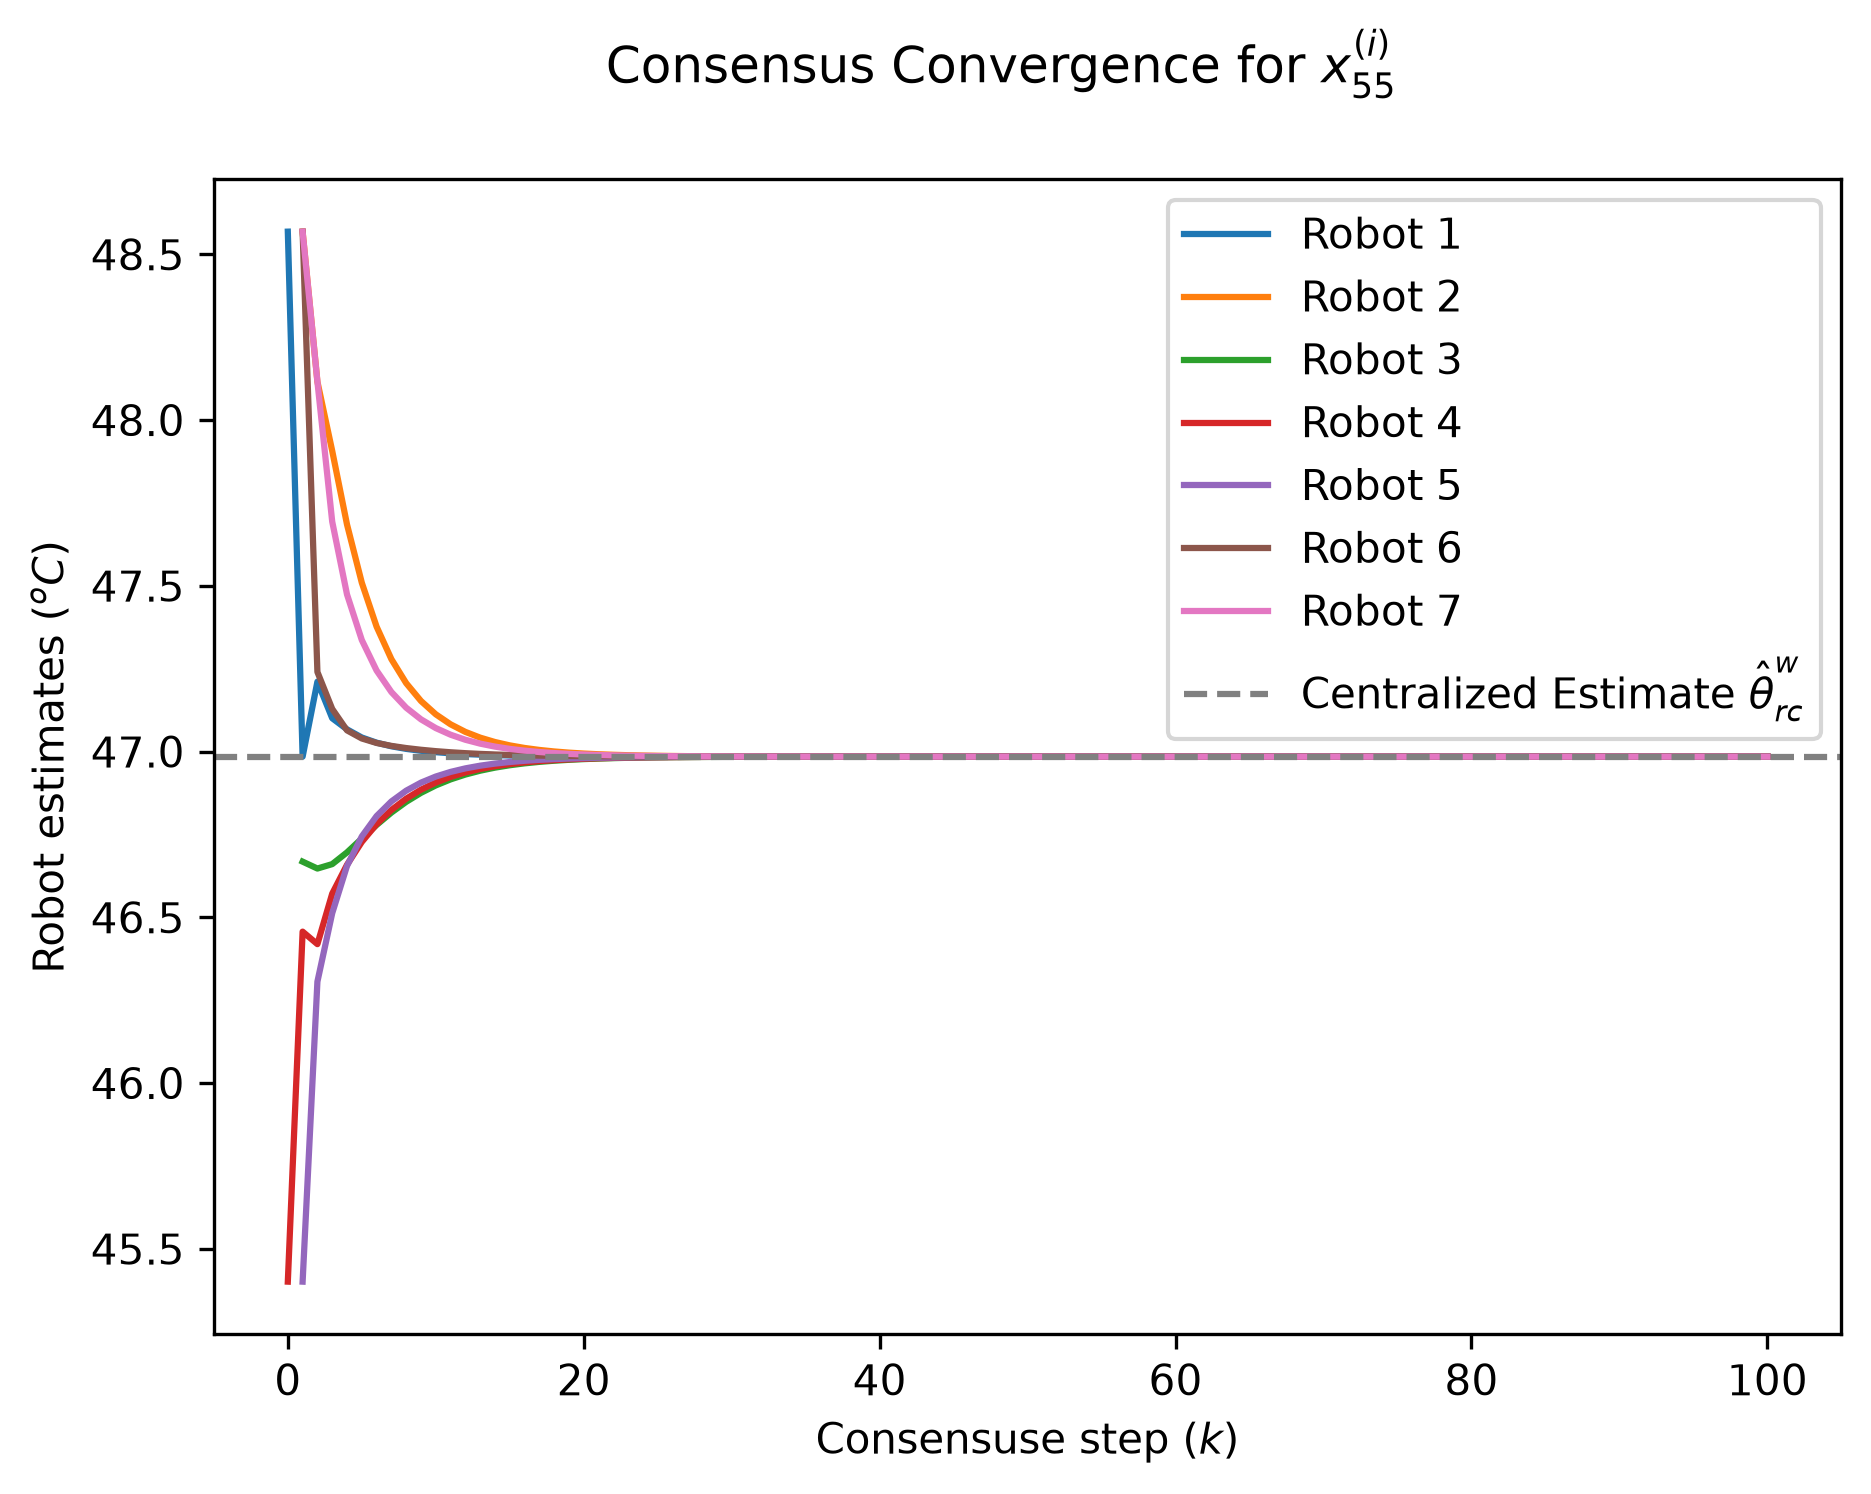
\includegraphics[width=0.5\textwidth]{Figures/x55_3_plot.png}
        \captionsetup{justification=centering}
        \caption{Estimated temperatures from all robots for cell (5,5) versus consensus step compared with theoretical centralized estimation from initial measurements.}
        \label{fig:x55_3_plot}
    \end{figure}

    \item Cooperation is \textit{crucial} for proper converge for each robot. If there was no cooperation across the network (as in no communication or transfer of information through it) then each robot's world map would be restricted to only the cells that they can directly measure and observe. They would have no means to obtain information outside of their sensing neighborhood. Cooperation also allows for greater \textit{accuracy} on shared cells within a robot's own neighborhood. As shown in Part 2(b), the variance (or uncertainty) in a the final consensus estimate for a cell is given in (\ref{eqn:varw})
    \begin{align*}
        \text{Var}(\hat\theta_{rc}^w)&=\frac1\Omega=\frac{1}{\sum_{i=1}^{n_{rc}}\frac{1}{\sigma_i^2}}.
    \end{align*}

    Because of this inverse of the sum of the inverse-variances, adding \textit{any} additional measurement, no matter \textit{how uncertain}, will improve the overall consensus variance. This can easily be demonstrated numerically. Let us use an example of two robots measuring a cell, one with a variance of 1 and the other with a variance of 100 (in arbitrary units). The combined uncertainty, when just considering robot 1, is
    \begin{align*}
        \text{Var}(\hat\theta_{rc}^w)&=\frac{1}{\frac11}=1,
    \end{align*}
    but if we then add robot 2's measurement, our new uncertainty becomes
    \begin{align*}
        \text{Var}(\hat\theta_{rc}^w)&=\frac{1}{\frac11+\frac1{100}}=\frac1{\frac{101}{100}}=\frac{100}{101}\approx0.99,
    \end{align*}
    which has improved, even though robot 2's measurement was very uncertain! Therefore, cooperation is \textit{only} beneficial to the accuracy of a cell's measurement, and the more robots that can measure a particular cell, the more accurate its result will be.
\end{enumerate}

\clearpage
\subsection*{}
\textbf{Comparison protocol for Parts 4 and 5.}
In the next two parts of the assignment we will compare performance of unweighted and uncertainty-weighted sensor fusion for two scenarios, one where there is a single very good sensor, and one where there is a single very bad sensor. To have a fair comparison, we will follow the following protocol.
Each robot will take one measurement of the map. Use the same measurement for both the weighted and the unweighted fusion scenario. In the two scenarios we will consider, robot 1 will be different from the rest. To examine effects of this heterogeneity, define the shared sensing region of robot 1 as
\begin{align*}
    \mathcal O_1&=\left\{(r,c):1\in\mathcal S_{rc},\ |\mathcal S_{rc}|\geq2\right\}.
\end{align*}
Intuitively, $\mathcal O_1$ contains the grid cell indices of all cells that are sensed by robot 1 that are also within sensing range of at least one other robot. 

To compare the unweighted and uncertainty-weighted fusion outcomes, we will plot both fused temperature maps and outline the cells in $\mathcal O_1$. Plot signed error maps $\hat\theta_{rc}-\theta_{rc}$ on $\mathcal O_1$, coloring cells outside it gray. To normalize the visual comparisons, use identical color limits to define your colormap: $10$--$50^oC$ for temperatures and $-15$--$15^oC$ for errors.

To compute error estimates, run 100 independent trials (a trial = measurement followed by rounds of consensus fusion), for each trial assuming no prior knowledge beyond measurement. Report MSE over all observed cells and over $\mathcal O_1$, averaging squared error over cells and trials. Also report RMSE=$\sqrt{\text{MSE}}$ on $\mathcal O_1$ in $^oC$, excluding unknown cells.

\subsection*{4.}
\textbf{One very accurate sensor.}
Set $\sigma_1^2=1(^oC)^2$ and $\sigma_i^2=225(^oC)^2$ for $i=2,\dots,7$: robot 1 has standard deviation $1^oC$ and the other six have standard deviation $15^oC$. Follow the comparison protocol above.
\begin{enumerate}[label=(\alph*)]
    \item On overlapping sensing neighborhoods, how much influence does robot 1 have under each method? Can ignoring uncertainty make fusion less accurate \textit{in expectation} than its measurement alone? Use the variance formulas from Part 2.
    \item Where can robot 1's accurate sensor improve the fused map?
\end{enumerate}

\noindent\textbf{ANSWER:}

Following the comparison protocol for Parts 4 and 5, the weighted versus unweighted fusion temperature maps are given in Figure \ref{fig:temperature_4}, and the weighted versus unweighted error maps of $\mathcal O_1$ are given in Figure \ref{fig:error_4}. 

As seen in Figure \ref{fig:temperature_4}, when using weighted estimates, the temperature estimates in $\mathcal V^{(1)}$ are very accurate. This is no surprise, as robot 1's variance was much lower than the other robots', and so its measurement was weighed much more heavily in the fusion consensus algorithm. Visually, the cells within $\mathcal V^{(1)}$ look nearly identical to those from Figure (\ref{fig:true_temperature_graph_network}) showing the true temperature field. However, outside of $\mathcal V^{(1)}$, the estimates are visually very inaccurate due to the high variance of the robots who could sense them. Therefore, while robot 1 was still able to make an accurate map of its own sensing neighborhood, it had to rely solely on the measurements of the uncertain other robots to form its map of the rest of the grid, leading to inaccuracy. However, in the \textit{unweighted} version, the final estimate of the cells within $\mathcal V^{(1)}$ are much less accurate due to the naive nature of averaging all robot measurements equally. This causes robot 1's accurate measurement to be lost in the uncertainty of the others, reducing the region's accuracy. The only exception to this is cell (3,4), which is in $\mathcal V^{(1)}$ but \textit{not} in $\mathcal O_1$ (i.e., \textit{only} robot 1 measures this cell). Because of this, robot 1 is not averaging its measurement with any other robots', and so it is able to remain accurate.

\begin{figure}[htb]
    \centering
    \begin{subfigure}[t]{0.45\textwidth}
        \centering
        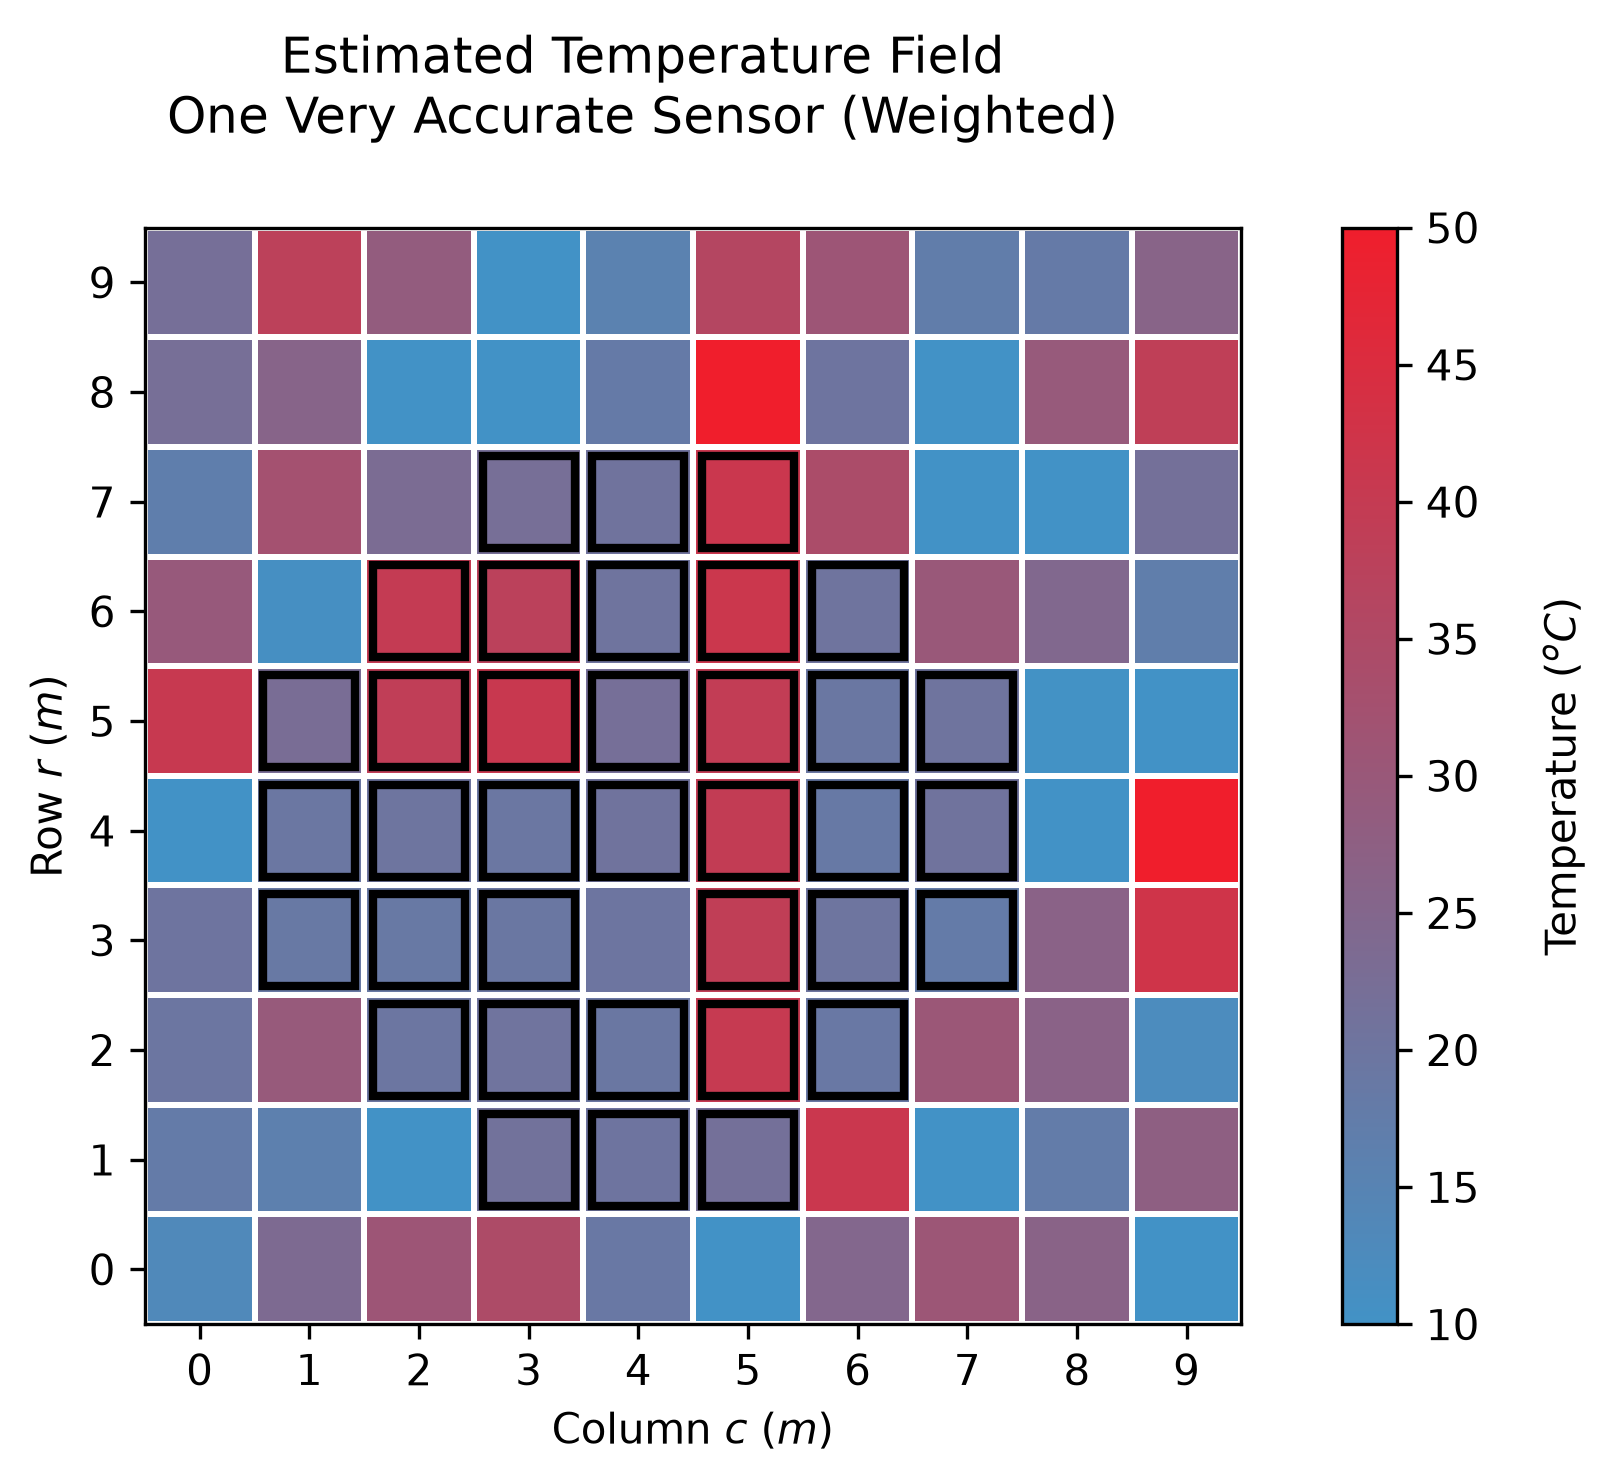
\includegraphics[width=\textwidth]{Figures/temperature_w_4.png}
        \captionsetup{justification=centering}
        \caption{Final total temperature map for weighted sensor fusion of measurements.}
        % \label{fig:}
    \end{subfigure}\hfill
    \begin{subfigure}[t]{0.45\textwidth}
        \centering
        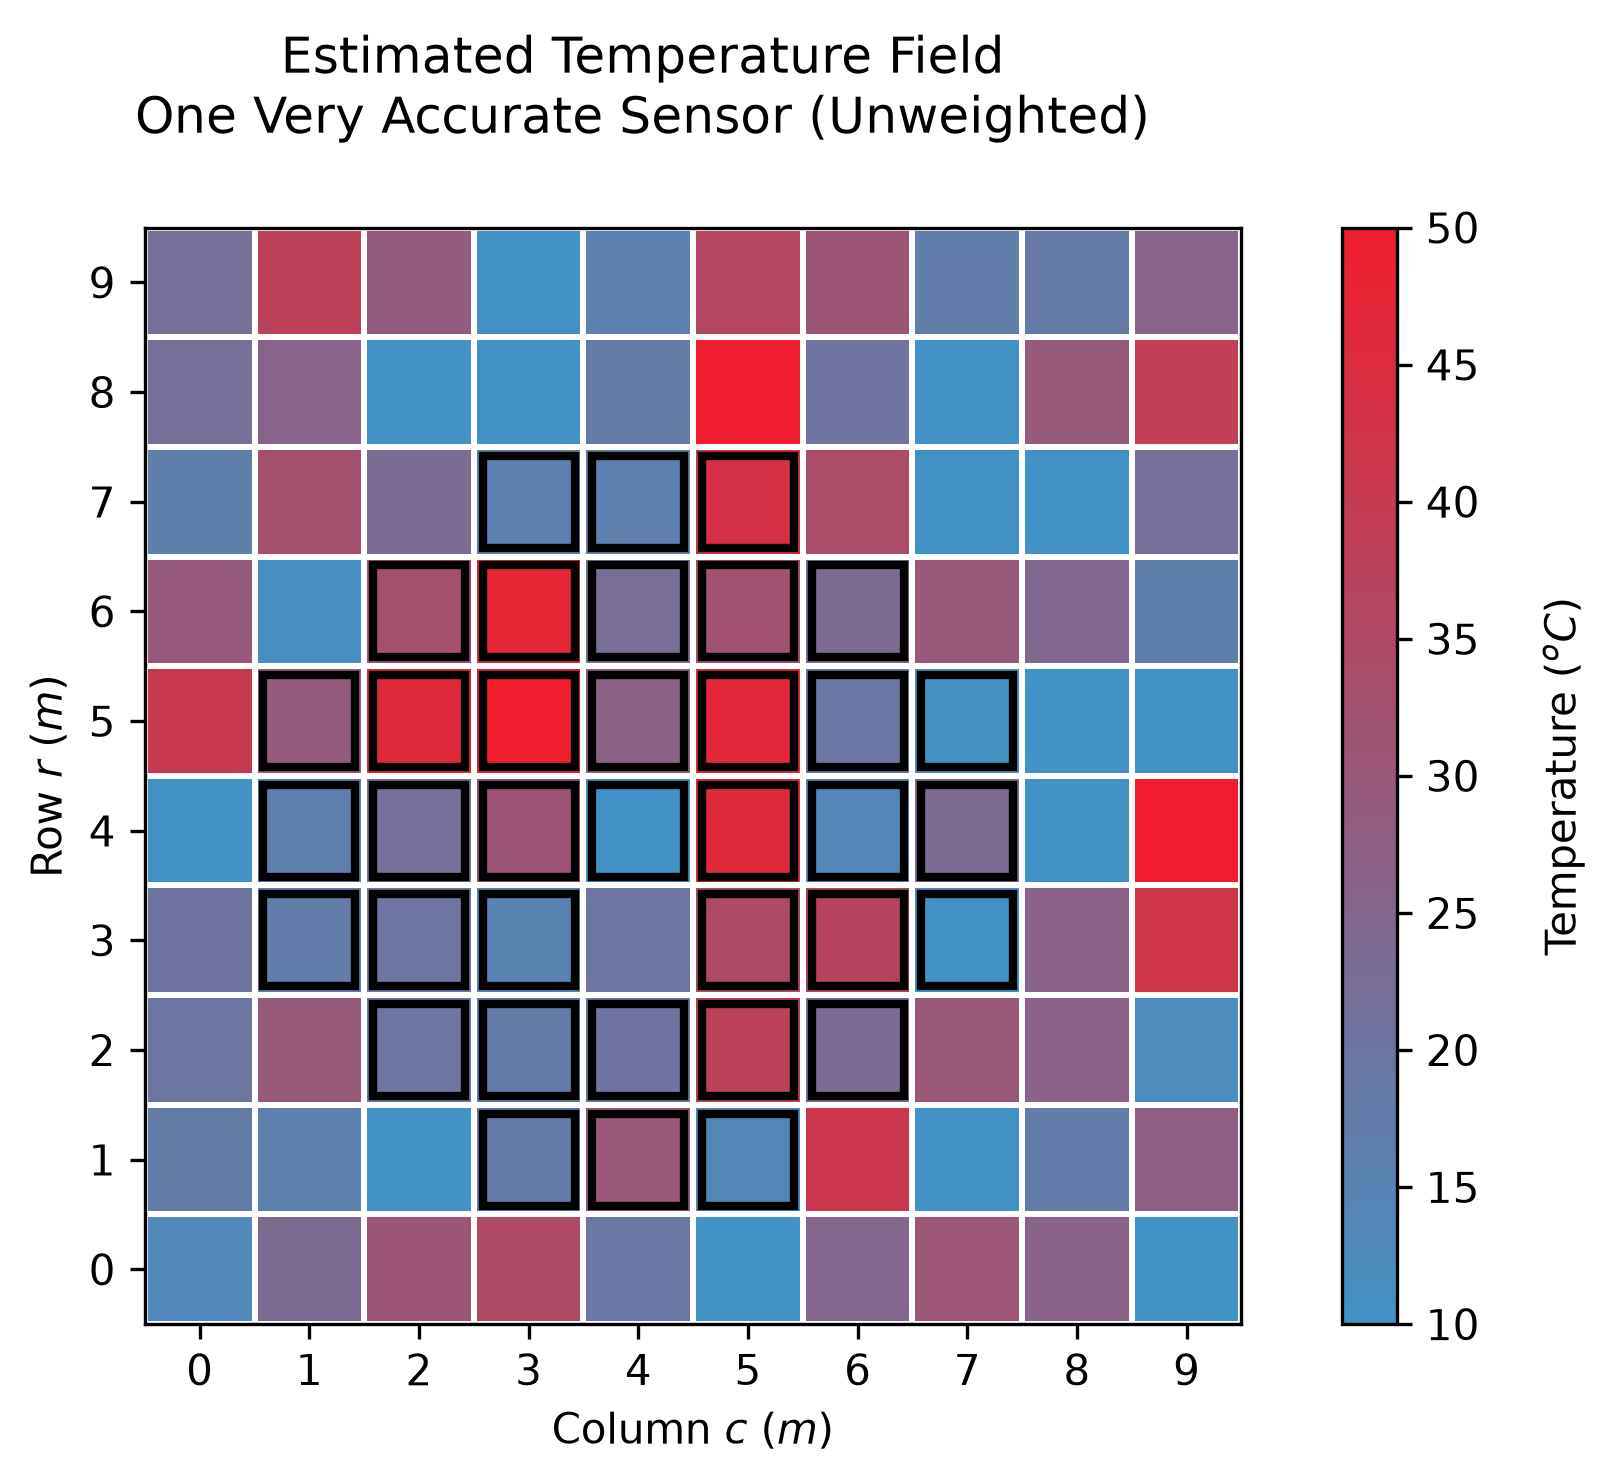
\includegraphics[width=\textwidth]{Figures/temperature_u_4.png}
        \captionsetup{justification=centering}
        \caption{Final total temperature field for unweighted sensor fusion of measurements.}
        % \label{fig:}
    \end{subfigure}
    \captionsetup{justification=centering}
    \caption{One very accurate sensor. Cells within $\mathcal O_1$ are bolded in a \textbf{black} square.}
    \label{fig:temperature_4}
\end{figure}

As seen in Figure \ref{fig:error_4}, the difference between the weighted and unweighted fusion algorithms is much more pronounced. The weighted estimate errors in $\mathcal O_1$ are all $\sim0$ with very little variance, while the unweighted estimate errors in $\mathcal O_1$ are much greater. This further exemplifies the issue of not properly weighting sensor measurements and accounting for measurement variance. If naively averaged, the final estimates can be very inaccurate, even in the region of a high-precision sensor.

\begin{figure}[htb]
    \centering
    \begin{subfigure}[t]{0.45\textwidth}
        \centering
        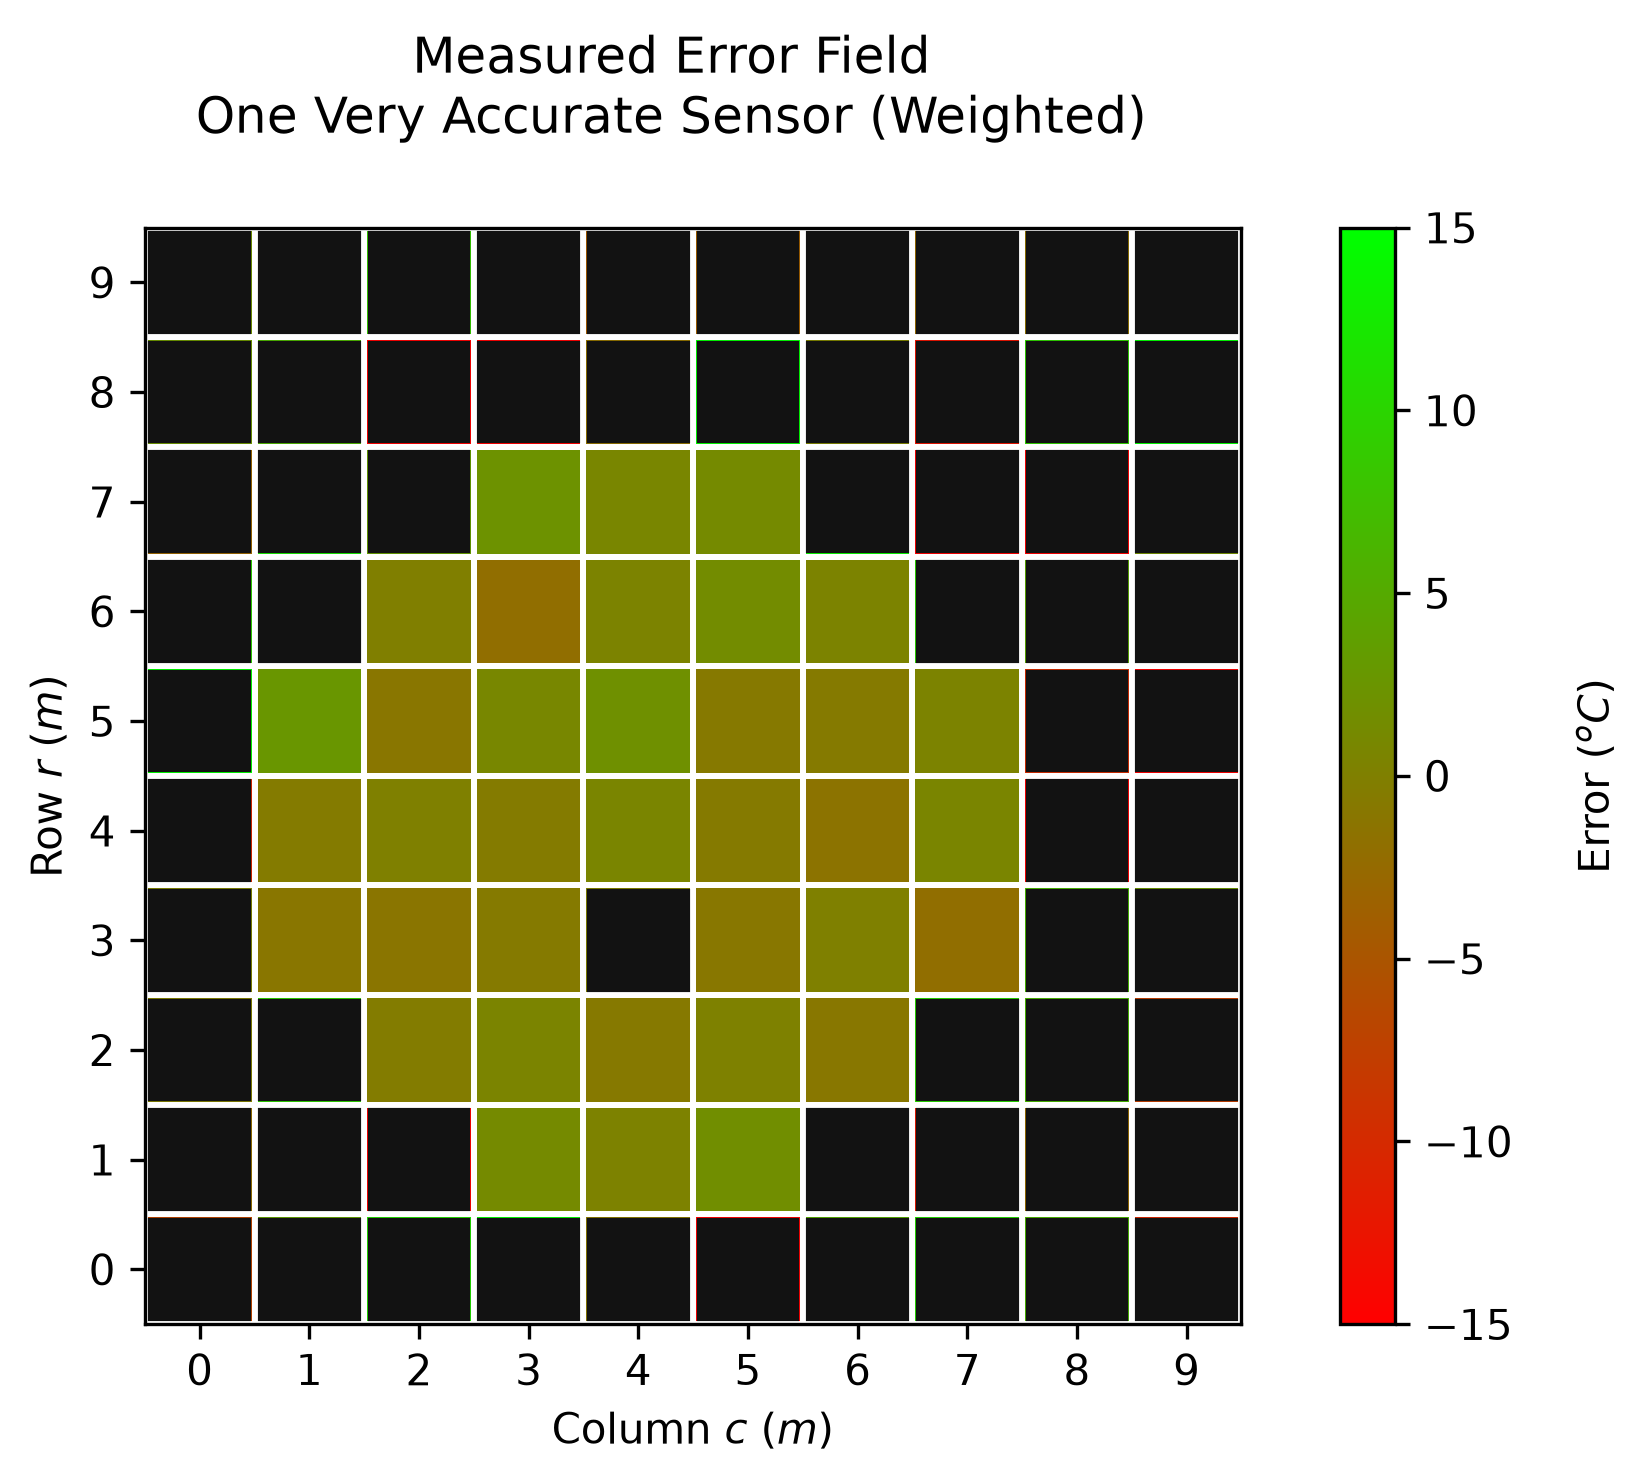
\includegraphics[width=\textwidth]{Figures/error_w_4.png}
        \captionsetup{justification=centering}
        \caption{Final error field of $\mathcal O_1$ for weighted sensor fusion of measurements.}
        % \label{fig:}
    \end{subfigure}\hfill
    \begin{subfigure}[t]{0.45\textwidth}
        \centering
        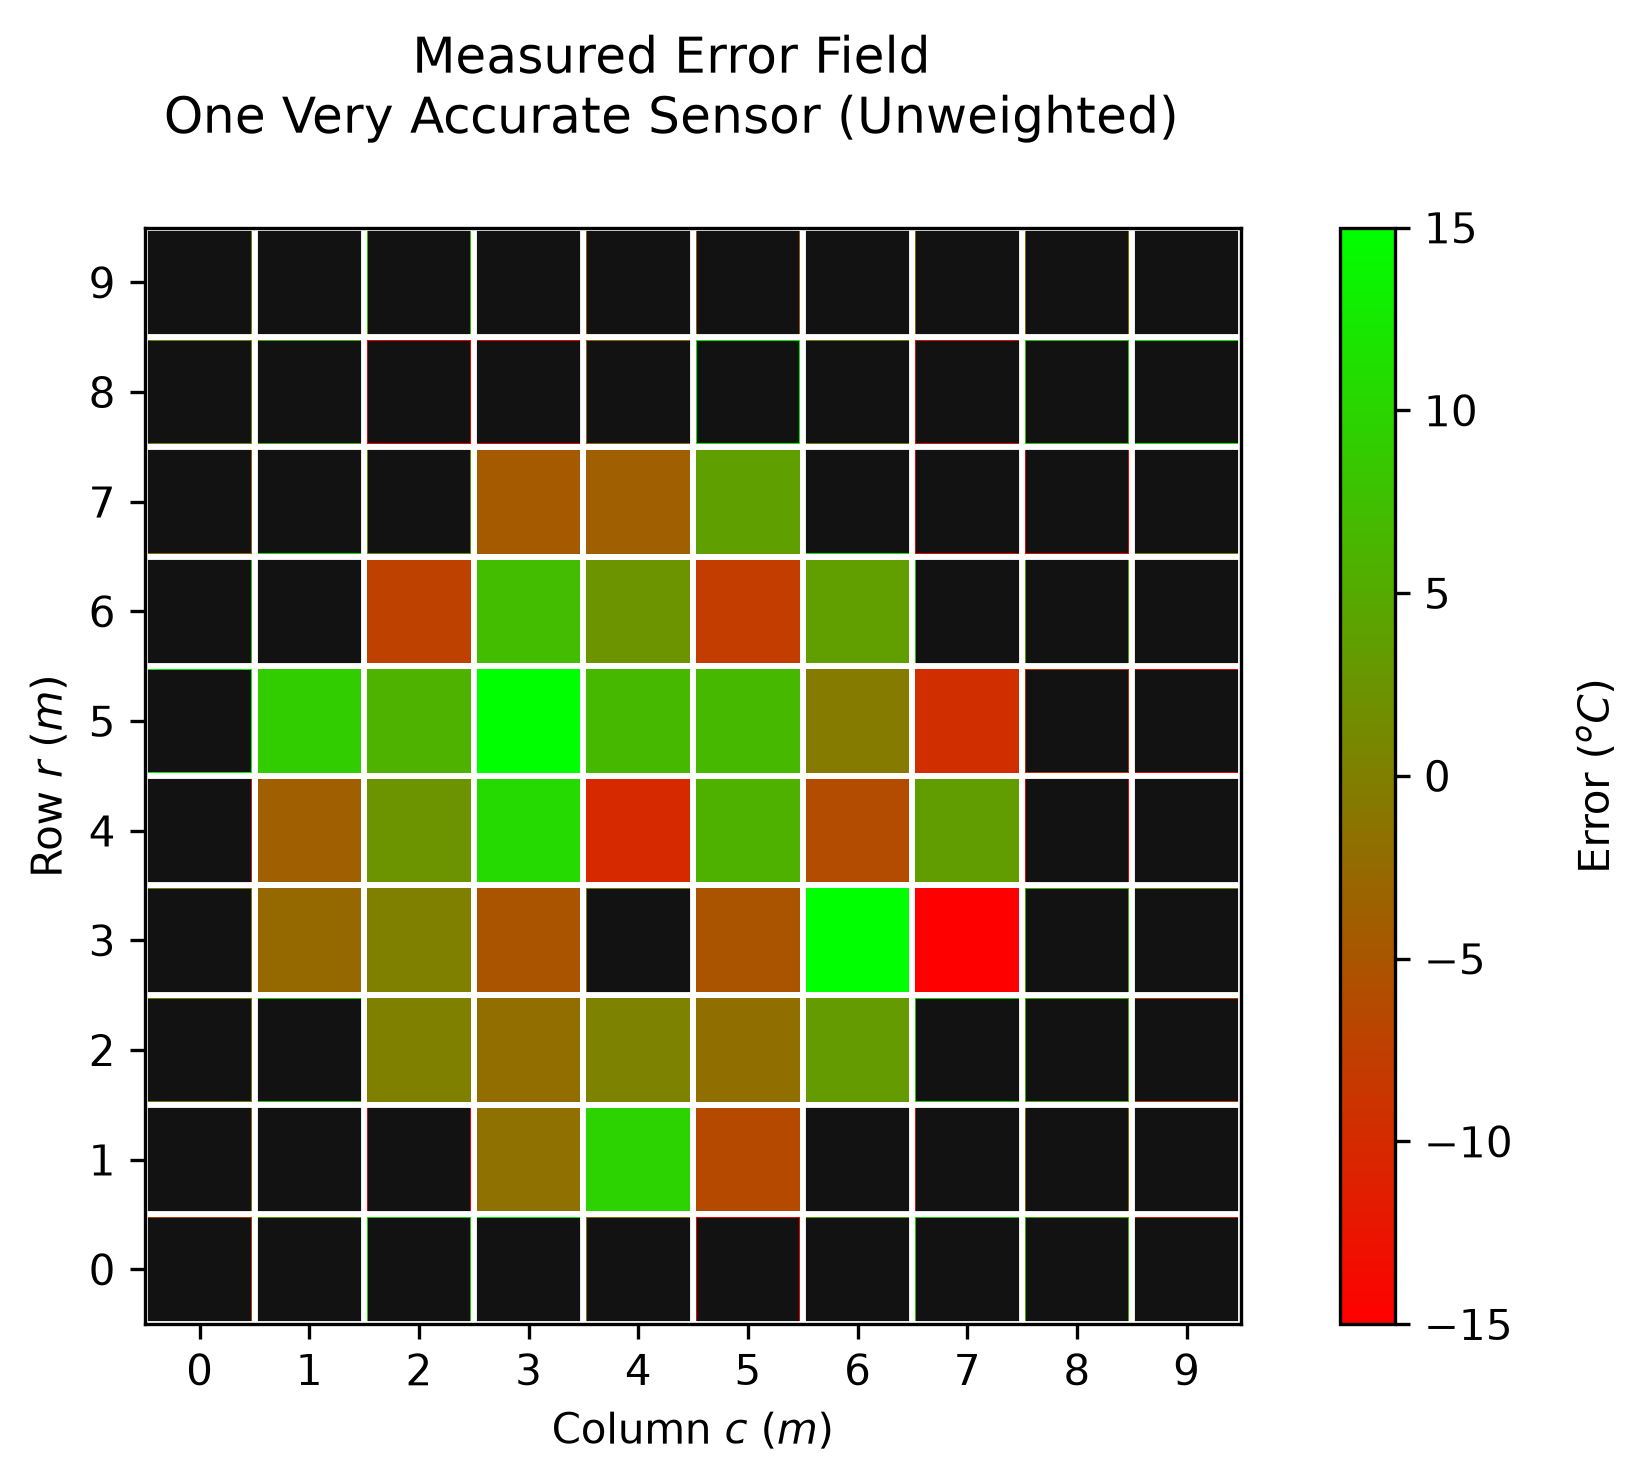
\includegraphics[width=\textwidth]{Figures/error_u_4.png}
        \captionsetup{justification=centering}
        \caption{Final error field of $\mathcal O_1$ for unweighted sensor fusion of measurements.}
        % \label{fig:}
    \end{subfigure}
    \captionsetup{justification=centering}
    \caption{One very accurate sensor.}
    \label{fig:error_4}
\end{figure}

Finally, over the course of 100 experiments, the estimated expected MSE of the entire field was calculated, as well as the MSE and RMSE of $\mathcal O_1$, for both the weighted and unweighted fusion algorithms. The results are given in Table \ref{tab:mse_4}. As seen, while the MSE in both the weighted and unweighted fusion for the \textit{entire} grid is high, within $\mathcal O_1$, the MSE and RMSE are much lower in the case of the weighted fusion. This is because robot 1 had direct measurement of the cells and, when given the opportunity to weight the measurements of the other robots appropriately, it was able to maintain an accurate estimate. However, when using the unweighted fusion, while the MSE in $\mathcal O_1$ is still improved compared to the total map, is is far less accurate.

\begin{table}[htb]
    \centering
    \caption{Comparison of field expected MSE, $\mathcal O_1$ MSE, and $\mathcal O_1$ RMSE for both weighted and unweighted sensor fusion methods.}
    \label{tab:mse_4}
    \begin{tabular}{m{0.2\textwidth}|M{0.2\textwidth}|M{0.2\textwidth}|M{0.2\textwidth}}
        \toprule
        \multicolumn{1}{c|}{\textbf{Fusion}} & $\widehat{\text{MSE}}$ all $(^oC)^2$ & $\widehat{\text{MSE}}$ $\mathcal O_1$ $(^oC)^2$ & $\widehat{\text{RMSE}}$ $\mathcal O_1$ $(^oC)$\\
        \midrule
        Weighted & 112.848 & 1.025 & 1.005\\
        Unweighted & 133.131 & 57.336 & 7.510\\
        \bottomrule
    \end{tabular}
\end{table}

\begin{enumerate}[label=(\alph*)]
    \item On its overlapping sensing neighborhoods ($\mathcal O_1$), robot 1, in the weighted situation, has a \textit{great} influence on the overall estimate of the cells within. As seen and mentioned in Table \ref{tab:mse_4}, ignoring uncertainty can make measurements less accurate in expectation than when robot 1 just uses its measurement alone. While in the weighted scenario in (\ref{eqn:varw}), adding measurements \textit{always} decreases the total uncertainty, in the unweighted scenario in (\ref{eqn:varu}), this is not strictly true. Once again, like as in Part 3(d), we will consider a robot with variance 1 and a robot with variance 100 (in arbitrary units)  and observe what happens when we fuse their measurements, except now in an \textit{unweighted} sense. With just robot 1, we have:
    \begin{align*}
        \text{Var}(\hat\theta_{rc}^u)&=\frac{1}{n_{rc}^2}\sum_{i=1}^{n_{rc}}\sigma_i^2=\frac1{1^2}(1)=1,
    \end{align*}
    but when fusing with robot 2, our variance then becomes
    \begin{align*}
        \text{Var}(\hat\theta_{rc}^u)&=\frac{1}{2^2}(1+100)=\frac{101}{4}=25.25.
    \end{align*}
    While this \textit{is} better than robot 2 could have done with its own measurement, it is worse than if robot 1 just simply ignored robot 2! Therefore, to properly fuse measurements, it must be done in an intelligent manner to avoid infecting measurements with large uncertainty.

    \item As seen in Figure \ref{fig:temperature_4}, robot 1's accurate measurement can only improve the total map \textit{in its own sensing neighborhood}. For the cells that are outside of its region, it can get no direct measurement, and so it \textit{must} reply on the measurements of others during the estimation.
\end{enumerate}

\clearpage
\subsection*{5.}
\textbf{One very inaccurate sensor.}
Set $\sigma_1^2=225(^oC)^2$ and $\sigma_i^21(^oC)^2$ for $i=2,\dots,7$ and repeat the comparison.
\begin{enumerate}[label=(\alph*)]
    \item On overlapping sensing neighborhoods, how does robot 1 affect each estimate? Compare the weighted estimator's variance with that obtained by discarding its reading. Does adding a correctly weighted, independent, unbiased reading with large variance necessarily reduce accuracy? \textit{Hint: after discarding a reading, renormalize the remaining estimator coefficients so they sum to one, then apply (\ref{eqn:gaussian_bv})}.
    \item Explain what happens on cells measured only by robot 1 and on cells outside its sensing range. Does agreement guarantee an accurate map?
\end{enumerate}

\noindent\textbf{ANSWER:}

Following the comparison protocol for Parts 4 and 5, the weighted versus unweighted fusion temperature maps are given in Figure \ref{fig:temperature_5}, and the weighted versus unweighted error maps of $\mathcal O_1$ are given in Figure \ref{fig:error_5}. 

As seen in Figure \ref{fig:temperature_5}, when using weighted estimates, the temperature estimates in $\mathcal V^{(1)}$ are very accurate, even \textit{despite} the large uncertainty of robot 1's measurement. This makes sense, as nearly every cell in $\mathcal V^{(1)}$ are being measured by at least one more robot, and their highly accurate measurement, when weighted with the measurement of robot 1, will create a very certain final estimate. The only exception to this is cell (3,4), which is in $\mathcal V^{(1)}$ but \textit{not} in $\mathcal O_1$. As seen, its estimate is \textit{not accurate}. As only robot 1 had a direct measurement of the cell, there were no other measurements to fuse with it and improve the accuracy. In the \textit{unweighted} version, however, we can see that while the rest of the map is accurate, $\mathcal V^{(1)}$ is \textit{not} accurate, even with the overlapping cells in $\mathcal O_1$. This is because the uncertain measurement from robot 1 is being improperly fused with the measurements from the other robots, leading to an overall \textit{increase} in uncertainty, rather than the decrease that occurs in the weighted case. For the cells outside of $\mathcal V^{(1)}$, no measurement from robot 1 is being fused, so no uncertainty is introduced.

\begin{figure}[htb]
    \centering
    \begin{subfigure}[t]{0.45\textwidth}
        \centering
        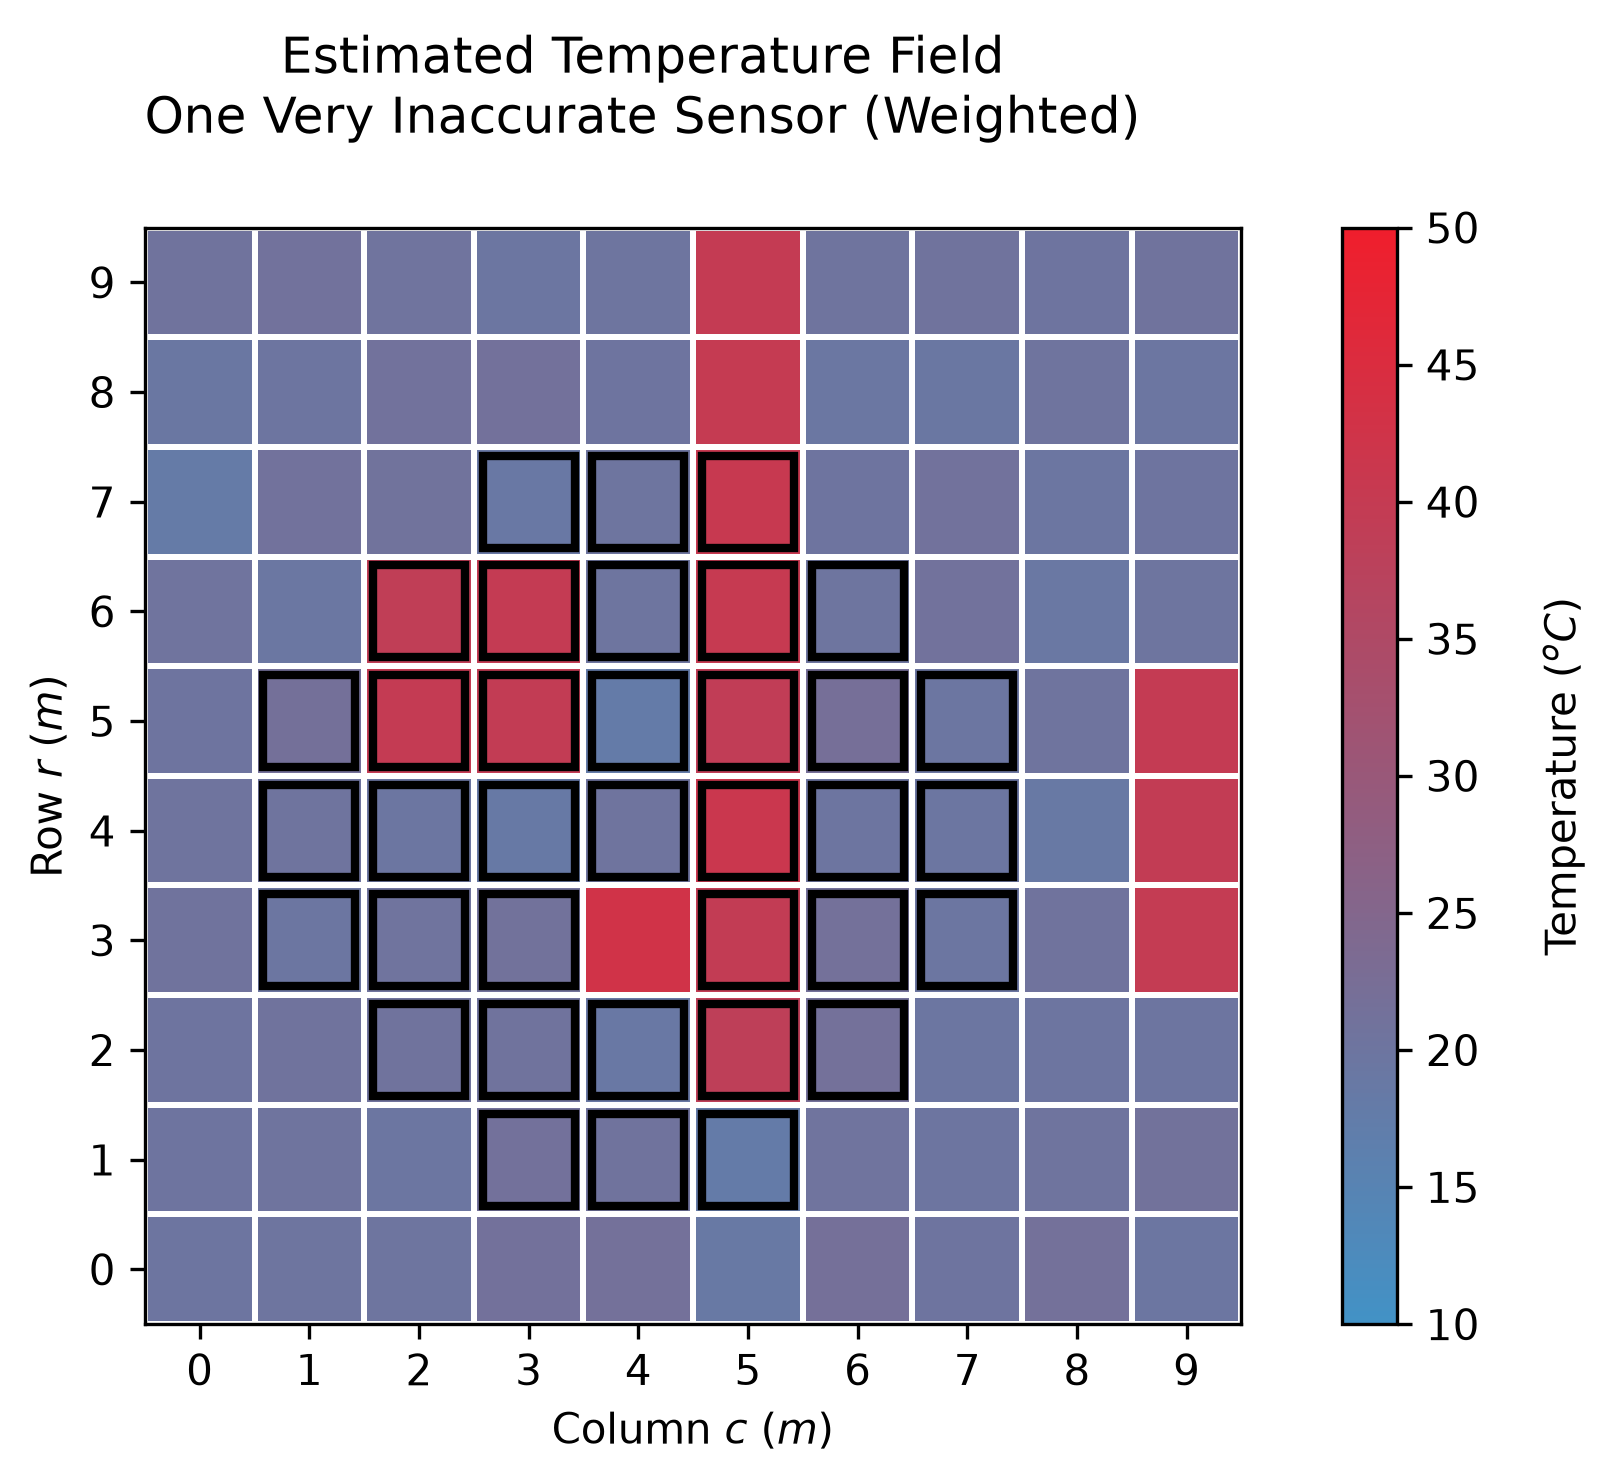
\includegraphics[width=\textwidth]{Figures/temperature_w_5.png}
        \captionsetup{justification=centering}
        \caption{Final total temperature map for weighted sensor fusion of measurements.}
        % \label{fig:}
    \end{subfigure}\hfill
    \begin{subfigure}[t]{0.45\textwidth}
        \centering
        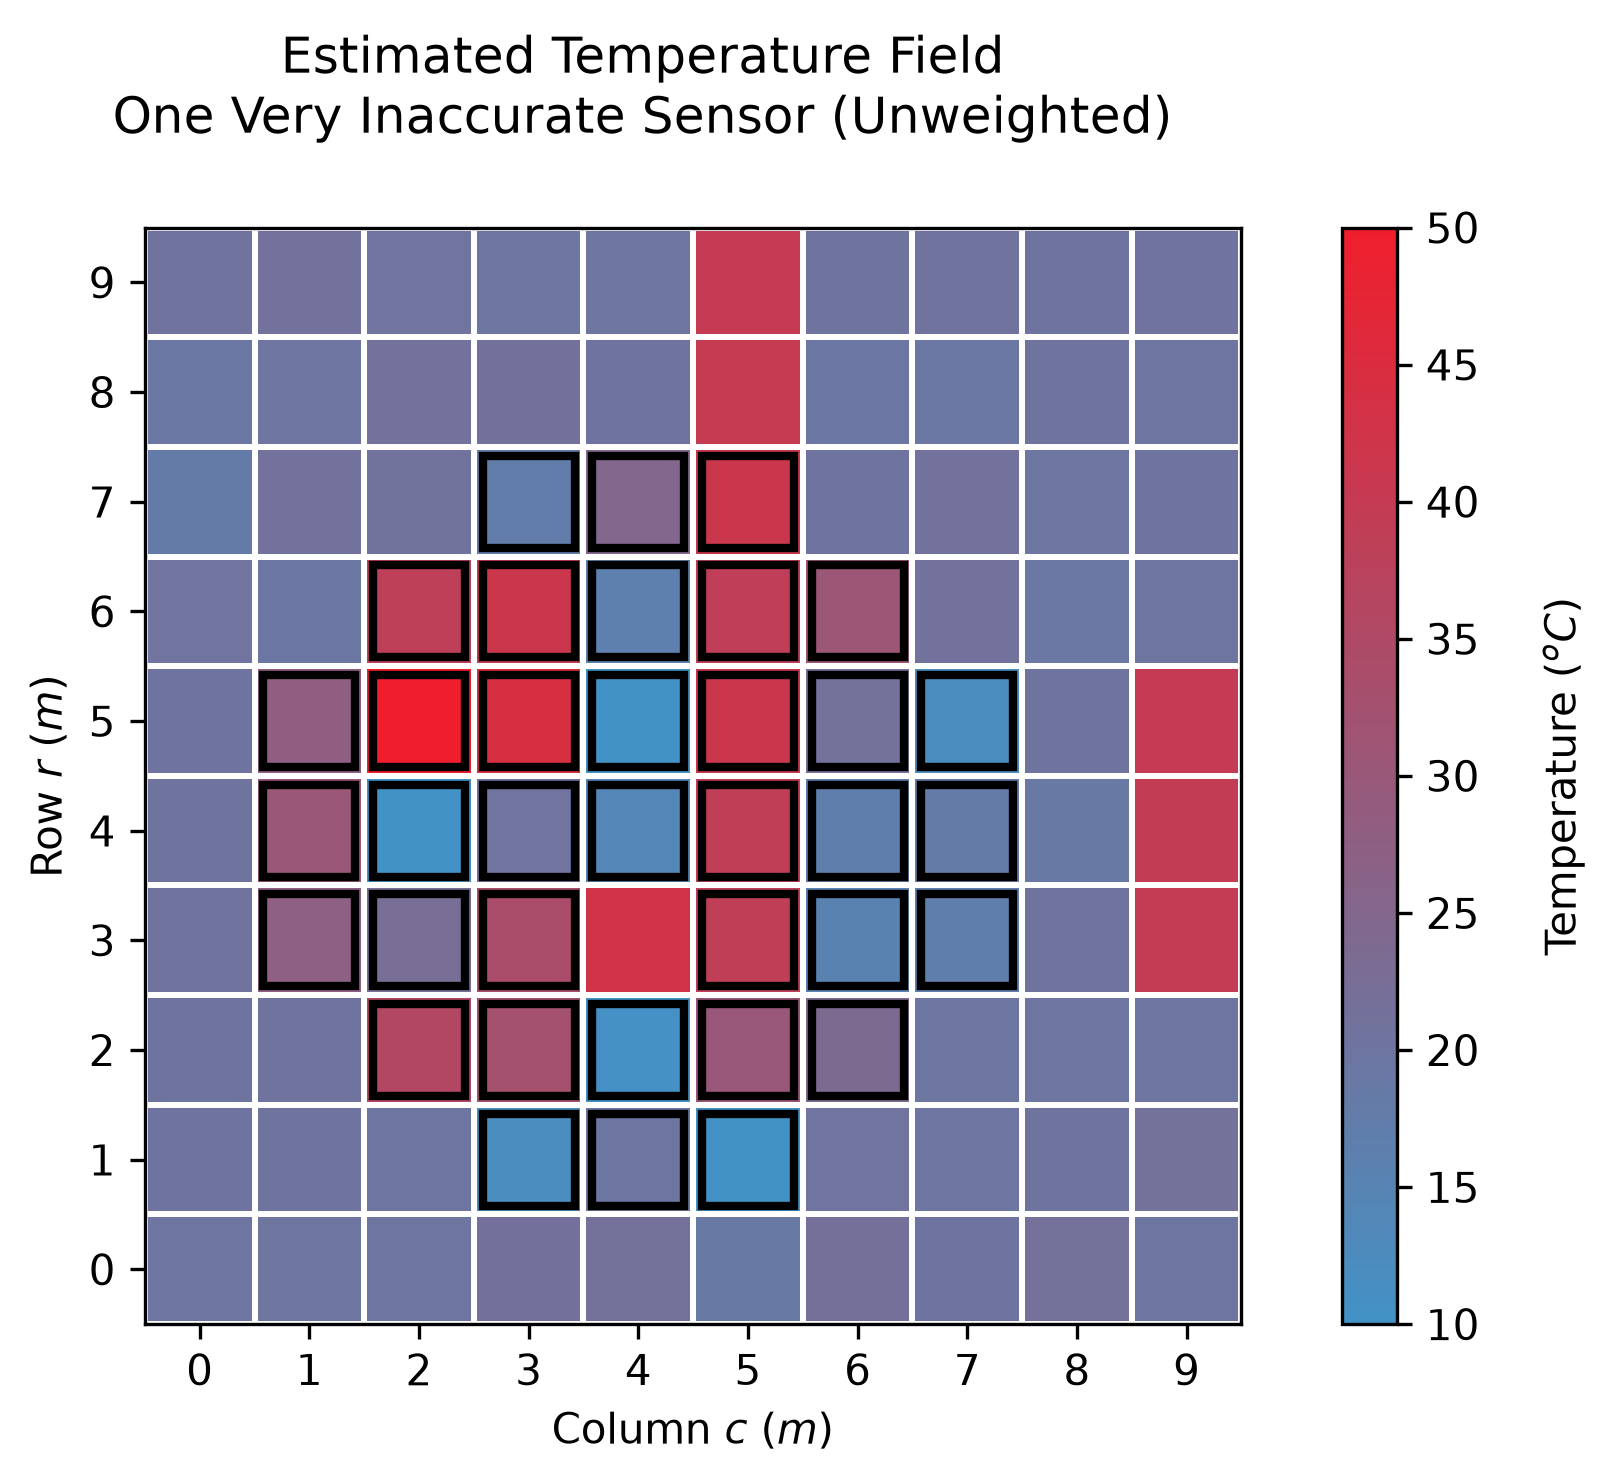
\includegraphics[width=\textwidth]{Figures/temperature_u_5.png}
        \captionsetup{justification=centering}
        \caption{Final total temperature field for unweighted sensor fusion of measurements.}
        % \label{fig:}
    \end{subfigure}
    \captionsetup{justification=centering}
    \caption{One very inaccurate sensor. Cells within $\mathcal O_1$ are bolded in a \textbf{black} square.}
    \label{fig:temperature_5}
\end{figure}

As seen in Figure \ref{fig:error_5}, the difference between the weighted and unweighted fusion algorithms is much more and is similar to what is seen in Figure \ref{fig:error_4}. The weighted estimate errors in $\mathcal O_1$ are all $\sim0$ with very little variance, while the unweighted estimate errors in $\mathcal O_1$ are much greater. Therefore, whenever there are highly uncertain measurements of a shared cell, they must be fused intelligently to avoid an increase in uncertainty from the more accurate measurements, as seen in the unweighted case.

\begin{figure}[htb]
    \centering
    \begin{subfigure}[t]{0.45\textwidth}
        \centering
        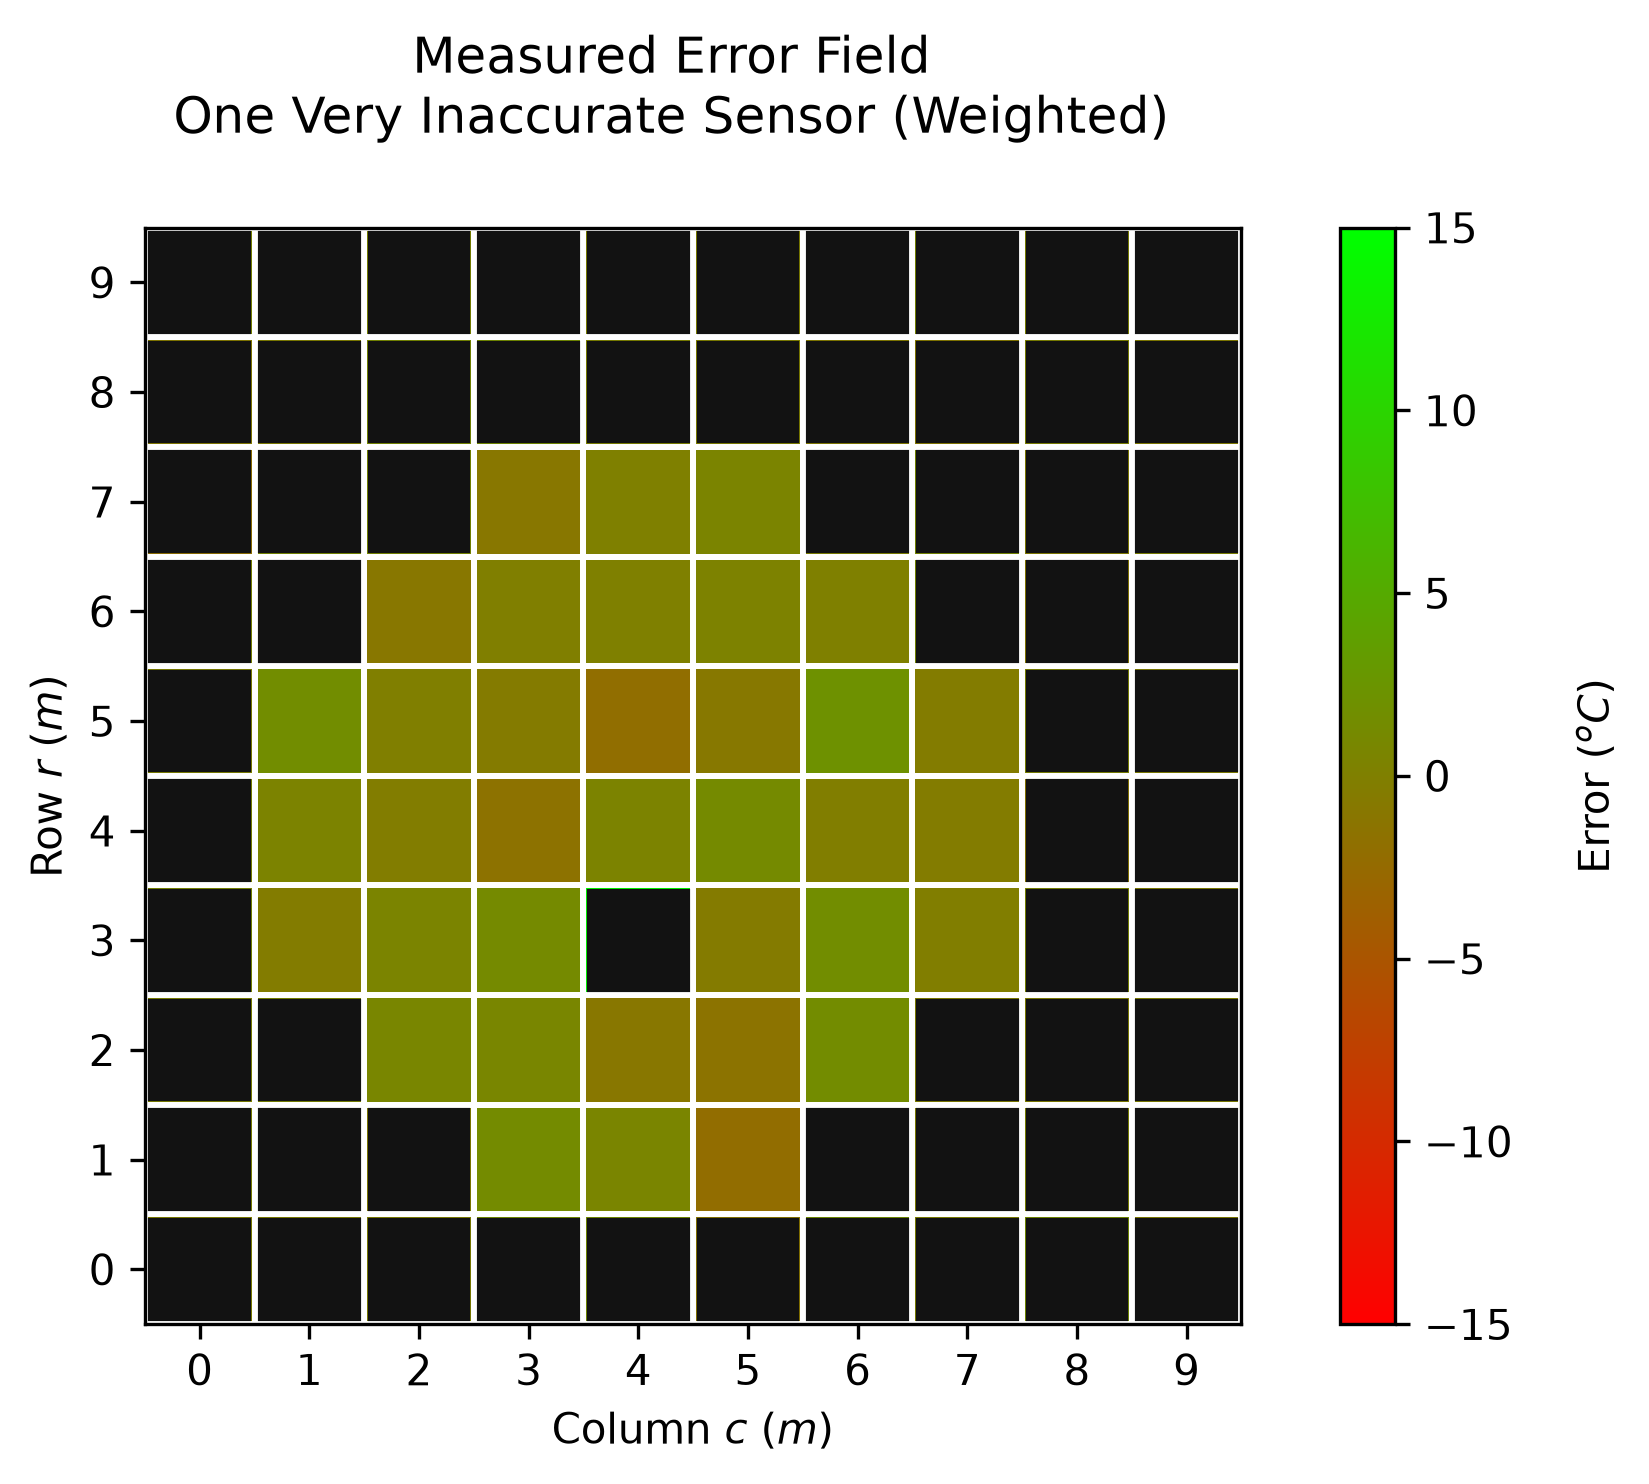
\includegraphics[width=\textwidth]{Figures/error_w_5.png}
        \captionsetup{justification=centering}
        \caption{Final error field of $\mathcal O_1$ for weighted sensor fusion of measurements.}
        % \label{fig:}
    \end{subfigure}\hfill
    \begin{subfigure}[t]{0.45\textwidth}
        \centering
        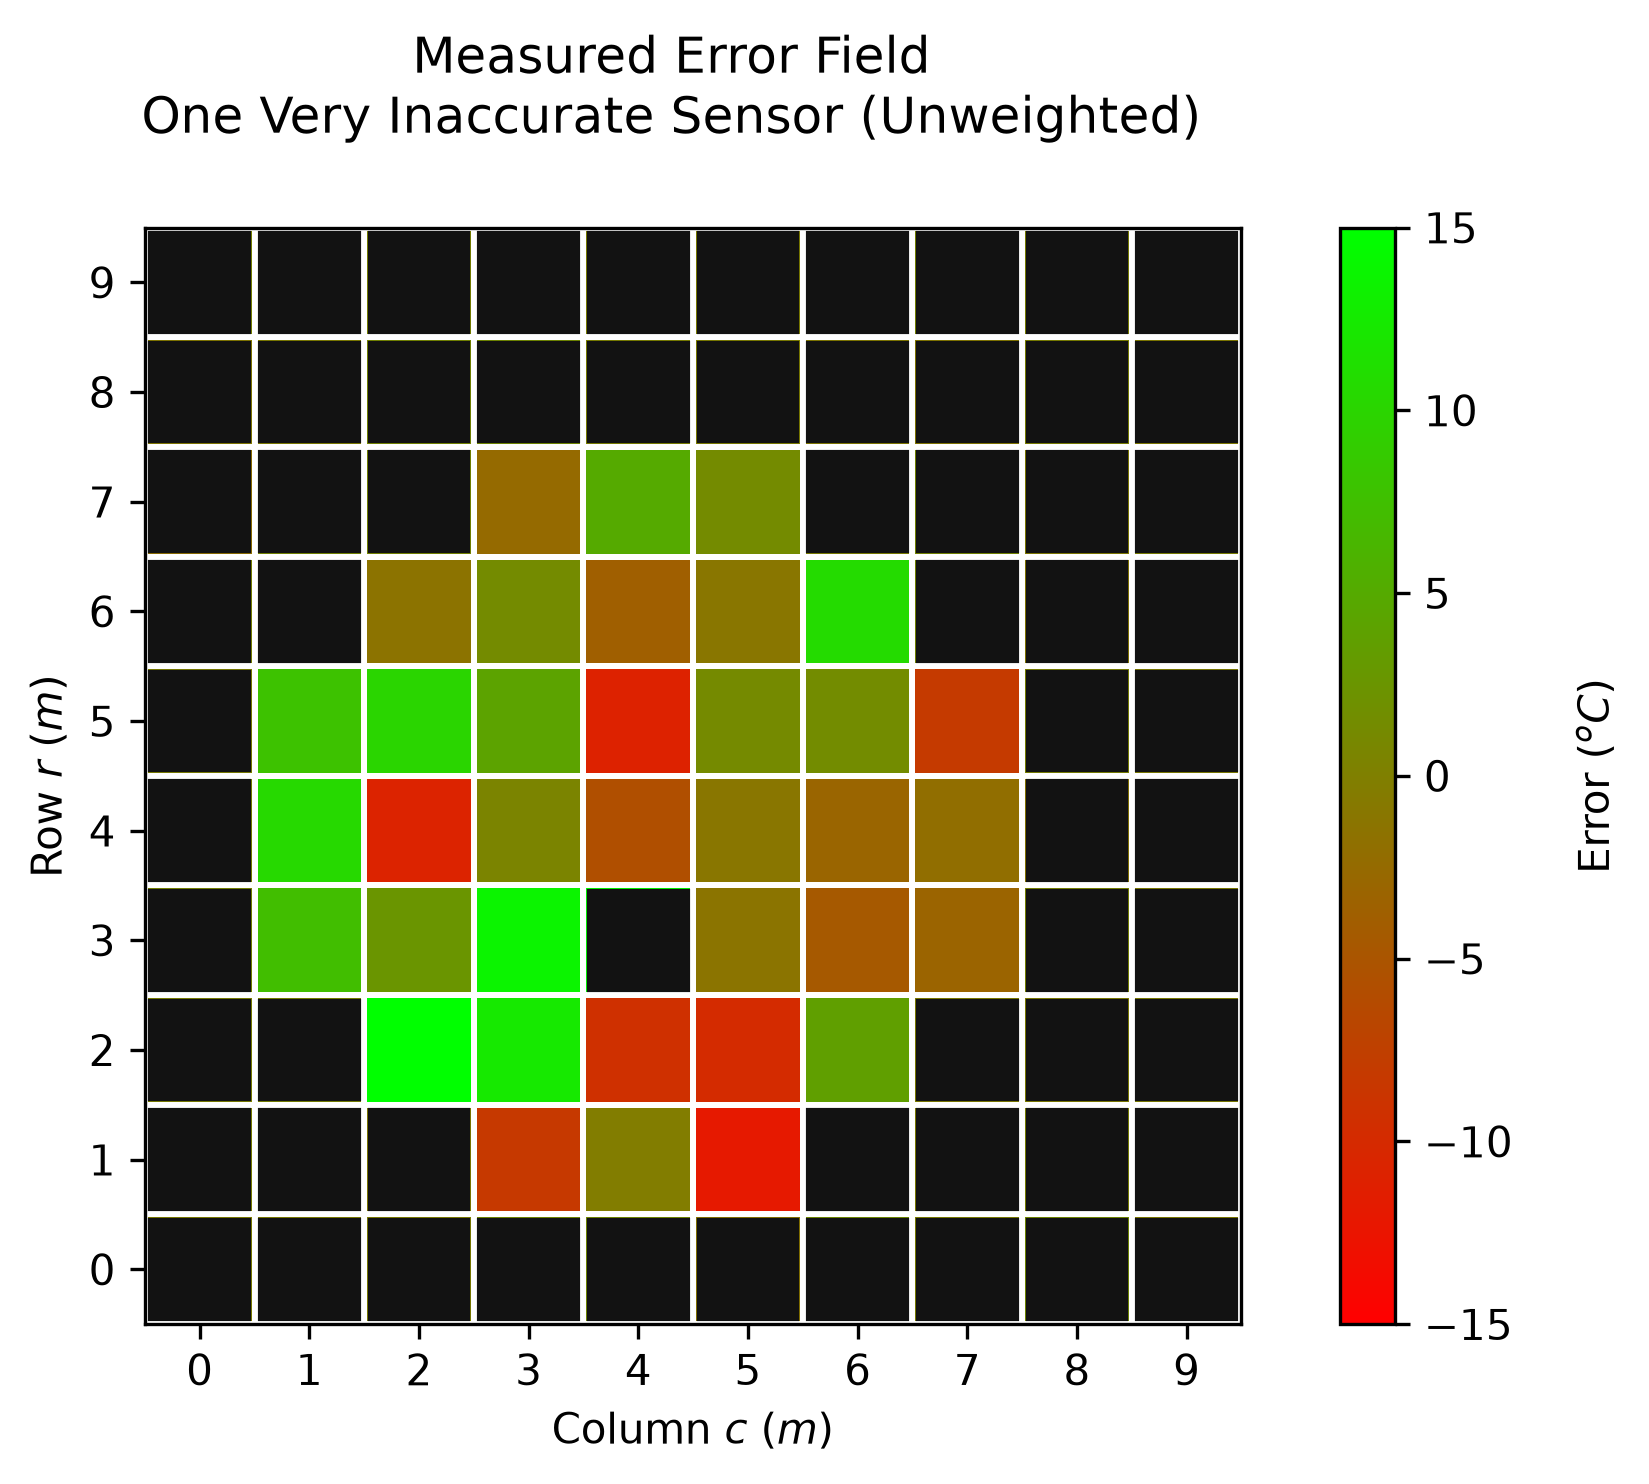
\includegraphics[width=\textwidth]{Figures/error_u_5.png}
        \captionsetup{justification=centering}
        \caption{Final error field of $\mathcal O_1$ for unweighted sensor fusion of measurements.}
        % \label{fig:}
    \end{subfigure}
    \captionsetup{justification=centering}
    \caption{One very inaccurate sensor.}
    \label{fig:error_5}
\end{figure}

Finally, over the course of 100 experiments, the estimated expected MSE of the entire field was calculated, as well as the MSE and RMSE of $\mathcal O_1$, for both the weighted and unweighted fusion algorithms. The results are given in Table \ref{tab:mse_5}. As seen, when using weighted fusion, the overall grid MSE, shared MSE, and shared RMSE are \textit{low}, as robot 1's uncertain measurement is able to be properly ``absorbed'' to improve the estimate, while with the unweighted fusion, the shared MSE is larger than the total grid MSE, showing the negative influence that robot 1's inaccurate sensor measurement had on the errors within the region. This is another demonstration of the importance of weighted fusion.

\begin{table}[htb]
    \centering
    \caption{Comparison of field expected MSE, $\mathcal O_1$ MSE, and $\mathcal O_1$ RMSE for both weighted and unweighted sensor fusion methods.}
    \label{tab:mse_5}
    \begin{tabular}{m{0.2\textwidth}|M{0.2\textwidth}|M{0.2\textwidth}|M{0.2\textwidth}}
        \toprule
        \multicolumn{1}{c|}{\textbf{Fusion}} & $\widehat{\text{MSE}}$ all $(^oC)^2$ & $\widehat{\text{MSE}}$ $\mathcal O_1$ $(^oC)^2$ & $\widehat{\text{RMSE}}$ $\mathcal O_1$ $(^oC)$\\
        \midrule
        Weighted & 3.203 & 0.635 & 0.791\\
        Unweighted & 16.852 & 38.548 & 6.160\\
        \bottomrule
    \end{tabular}
\end{table}

\begin{enumerate}[label=(\alph*)]
    \item On the overlapping neighborhood $\mathcal O_1$, whether or not robot 1's measurement affects the final variance in a positive or negative way is entirely dependent on if the fusion is weighted or unweighted. As described in Part 3(d), when using weighted fusion, \textit{any} new independent, unbiased measurement, no matter how poor, will improve the fused uncertainty, while in the unweighted case, as demonstrated in Part 4(a), can actually \textit{increase} the fused uncertainty. To demonstrate this again, we can consider (\ref{eqn:varw}) both when robot 1 is included and when robot 1's measurement is discarded. With robot 1 included, the fused variance follows exactly (\ref{eqn:varw}):
    \begin{align*}
        \text{Var}(\hat\theta_{rc}^w)&=\frac{1}{\sum_{i=1}^{n_{rc}}\frac{1}{\sigma_i^2}}=\frac{1}{\frac{1}{\sigma_1^2}+\frac{1}{\sigma_2^2}+\dots+\frac{1}{\sigma_{n_{rc}}^2}}=\frac{1}{\frac{1}{\sigma_1^2}+\sum_{i=2}^{n_{rc}}\frac{1}{\sigma_i^2}},
    \end{align*}
    and if we remove one robot and re-normalize, we have,
    \begin{align*}
        \text{Var}^*(\hat\theta_{rc}^w)&=\frac{1}{\frac{1}{\sigma_2^2}+\dots+\frac{1}{\sigma_{n_{rc}}^2}}=\frac{1}{\sum_{i=2}^{n_{rc}}\frac{1}{\sigma_i^2}}.
    \end{align*}

    Therefore, we can say $\frac{1}{\sigma_1^2}=a>0$ and $\sum_{i=2}^{n_{rc}}\frac{1}{\sigma_i^2}=b>0$, so our comparison is then
    \begin{align*}
        \text{Var}(\hat\theta_{rc}^w)&<\text{Var}^*(\hat\theta_{rc}^w)\\
        \frac{1}{a+b}&<\frac{1}{b}\ \forall a,
    \end{align*}
    so no matter how poor robot 1's measurement is, it will always improve the estimated fused uncertainty for weighted fusion. However, for unweighted fusion, we have, from (\ref{eqn:varu}), with robot 1 included,
    \begin{align*}
        \text{Var}(\hat\theta_{rc}^u)&=\frac{1}{n_{rc}^2}\sum_{i=1}^{n_{rc}}\sigma_i^2=\frac{1}{n_{rc}^2}\left(\sigma_1^2+\sum_{i=2}^{n_{rc}}\sigma_i^2\right),
    \end{align*}
    and without robot 1 included,
    \begin{align*}
        \text{Var}^*(\hat\theta_{rc}^u)&=\frac{1}{(n_{rc}-1)^2}\sum_{i=2}^{n_{rc}}\sigma_i^2.
    \end{align*}

    Let us call $\sum_{i=2}^{n_{rc}}\sigma_i^2=a>0$ and compare the relative size. If we want the addition of robot 1 to decrease the uncertainty, then we need to satisfy the ratio:
    \begin{align*}
        \frac{\text{Var}(\hat\theta_{rc}^w)}{\text{Var}^*(\hat\theta_{rc}^u)}&<1\\
        \frac{\frac{\sigma_1^2+a}{n_{rc}^2}}{\frac{a}{(n_{rc}-1)^2}}&<1\\
        \frac{(\sigma_1^2+a)(n_{rc}-1)^2}{an_{rc}^2}&<1\\
        \frac{\sigma_1^2+a}{a}<\frac{n_{rc}^2}{(n_{rc}-1)^2},
    \end{align*}
    which shows that adding a measurement with uncertainty $\sigma_1^2$ only \textit{improves} the overall uncertainty if it is sufficiently small such that the ratio is less than $\frac{n_{rc}^2}{(n_{rc}-1)^2}$. In the case of this example, when $\sigma_1^2=255\ (^oC)^2$, the ratio is violated as, in the best case for $n_{rc}=2$, we have,
    \begin{align*}
        \frac{255+1}{1}\nless\frac{4}{1}.
    \end{align*}

    \item For cells only measured by robot 1, as seen in Figure \ref{fig:temperature_5}, they remain highly uncertain, as there are no accurate measurements to properly fuse them with. However, for the \textit{rest} of the map that robot 1 does not directly measure, the estimates are highly accurate, as they fused only the accurate robot measurements. Therefore, even in the case of weighted sensor fusion, the final agreement does \textit{not} necessary guarantee a totally accurate temperature map, as if a region is only measured by a highly uncertain sensor, the final estimates will remain highly uncertain in finality.
\end{enumerate}

\clearpage
\subsection*{6.}
\textbf{Sequential measurements.}
Return to the \textit{one very accurate sensor} scenario from Part 4: $\sigma_1^2=1$ and $\sigma_i^2=225$ for $i=2,\dots,7$, in $(^oC)^2$. Treat its single sensing round as $t=1$, then collect independent new measurements at $t=2,\dots,20$. Keep the temperature field, robot locations, sensing neighborhoods, and communication graph fixed.

Extend your code to implement sequential measurement updates. Let $m_{irc}=1$ if robot $i$ measures cell $(r,c)$ and 0 otherwise. Write $y_{irc}(t)$ for its measurement, using zero as a placeholder for unobserved cells. Initialize $H_{irc}(0)=J_{irc}(0)=S_{irc}(0)=C_{irc}(0)$.

For uncertainty-weighted fusion, update
\begin{align*}
    H_{irc}(t)&=H_{irc}(t-1)+m_{irc}\frac{y_{irc}(t)}{\sigma_i^2},\\
    J_{irc}(t)&=J_{irc}(t-1)+\frac{m_{irc}}{\sigma_i^2}.
\end{align*}
For unweighted fusion, update
\begin{align*}
    S_{irc}(t)&=S_{irc}(t-1)+m_{irc}y_{irc}(t)\\
    C_{irc}(t)&=C_{irc}(t-1)+m_{irc}
\end{align*}

At each sensing time $t$, copy $H_{irc}(t), J_{irc}(t)$ into the numerator and denominator consensus states for weighted fusion, or $S_{irc}(t), C_{irc}(t)$ for unweighted fusion. Run $K=100$ communication rounds using the discrete-time consensus protocol in between each new measurement. 

Implement both the unweighted and the uncertainty-weighted fusion strategies, running $K=100$ communication rounds after each sensing round. Over 100 independent experiments, plot MSE against $t$ for both methods, separately over all observed cells and over $\mathcal O_1$.

For one experiment, also compare the shared map estimate after \textit{one sensing round} $(t=1)$ with the estimate after \textit{20 sensing rounds} $(t=20)$, using all measurements collected through each time. Show both unweighted and uncertainty-weighted results (four maps total), using the same robot's estimate after consensus and the same measurements for both methods. Use a common 10--$50^oC$ color scale, label all row and column indices, and outline $\mathcal O_1$. Briefly discuss how the visual improvement relates to the MSE plots.

\vspace{\baselineskip}
\noindent\textbf{ANSWER:}
The MSE against $t$ for sequential sensor measurements for both weighted and unweighted uncertainty strategies across the total grid and across $\mathcal O_1$ are given in Figure \ref{fig:mse_plot}. As seen, in \textit{all} cases, the MSE decreases as more sequential measurements are included into the final estimate. This is expected, as for a single individual cell, the expected value in infinitum is the maximum likelihood value from (\ref{eqn:theta_w}) or (\ref{eqn:theta_u}) of the \textit{expected} measurements $\mathbb E(\theta_{irc}$, rather than of the measurements themselves. And, as seen when calculating the bias in Part 3(b) (\ref{eqn:bw}) and (\ref{eqn:bu}), this is exactly the true temperature value of the cell! So, no matter \textit{what} fusion strategy, repeated measurements \textit{will} converge to the true temperature when fused, which is exactly what is seen in the Figure. However, using a \textit{weighted} fusion method for repeated measurements ensures that the true temperature is converged to much quicker (at least in the regions with accurate sensors, such as $\mathcal O_1$). In regions outside of $\mathcal O_1$, the fusion method had little bearing on the convergence results.

\begin{figure}[htb]
    \centering
    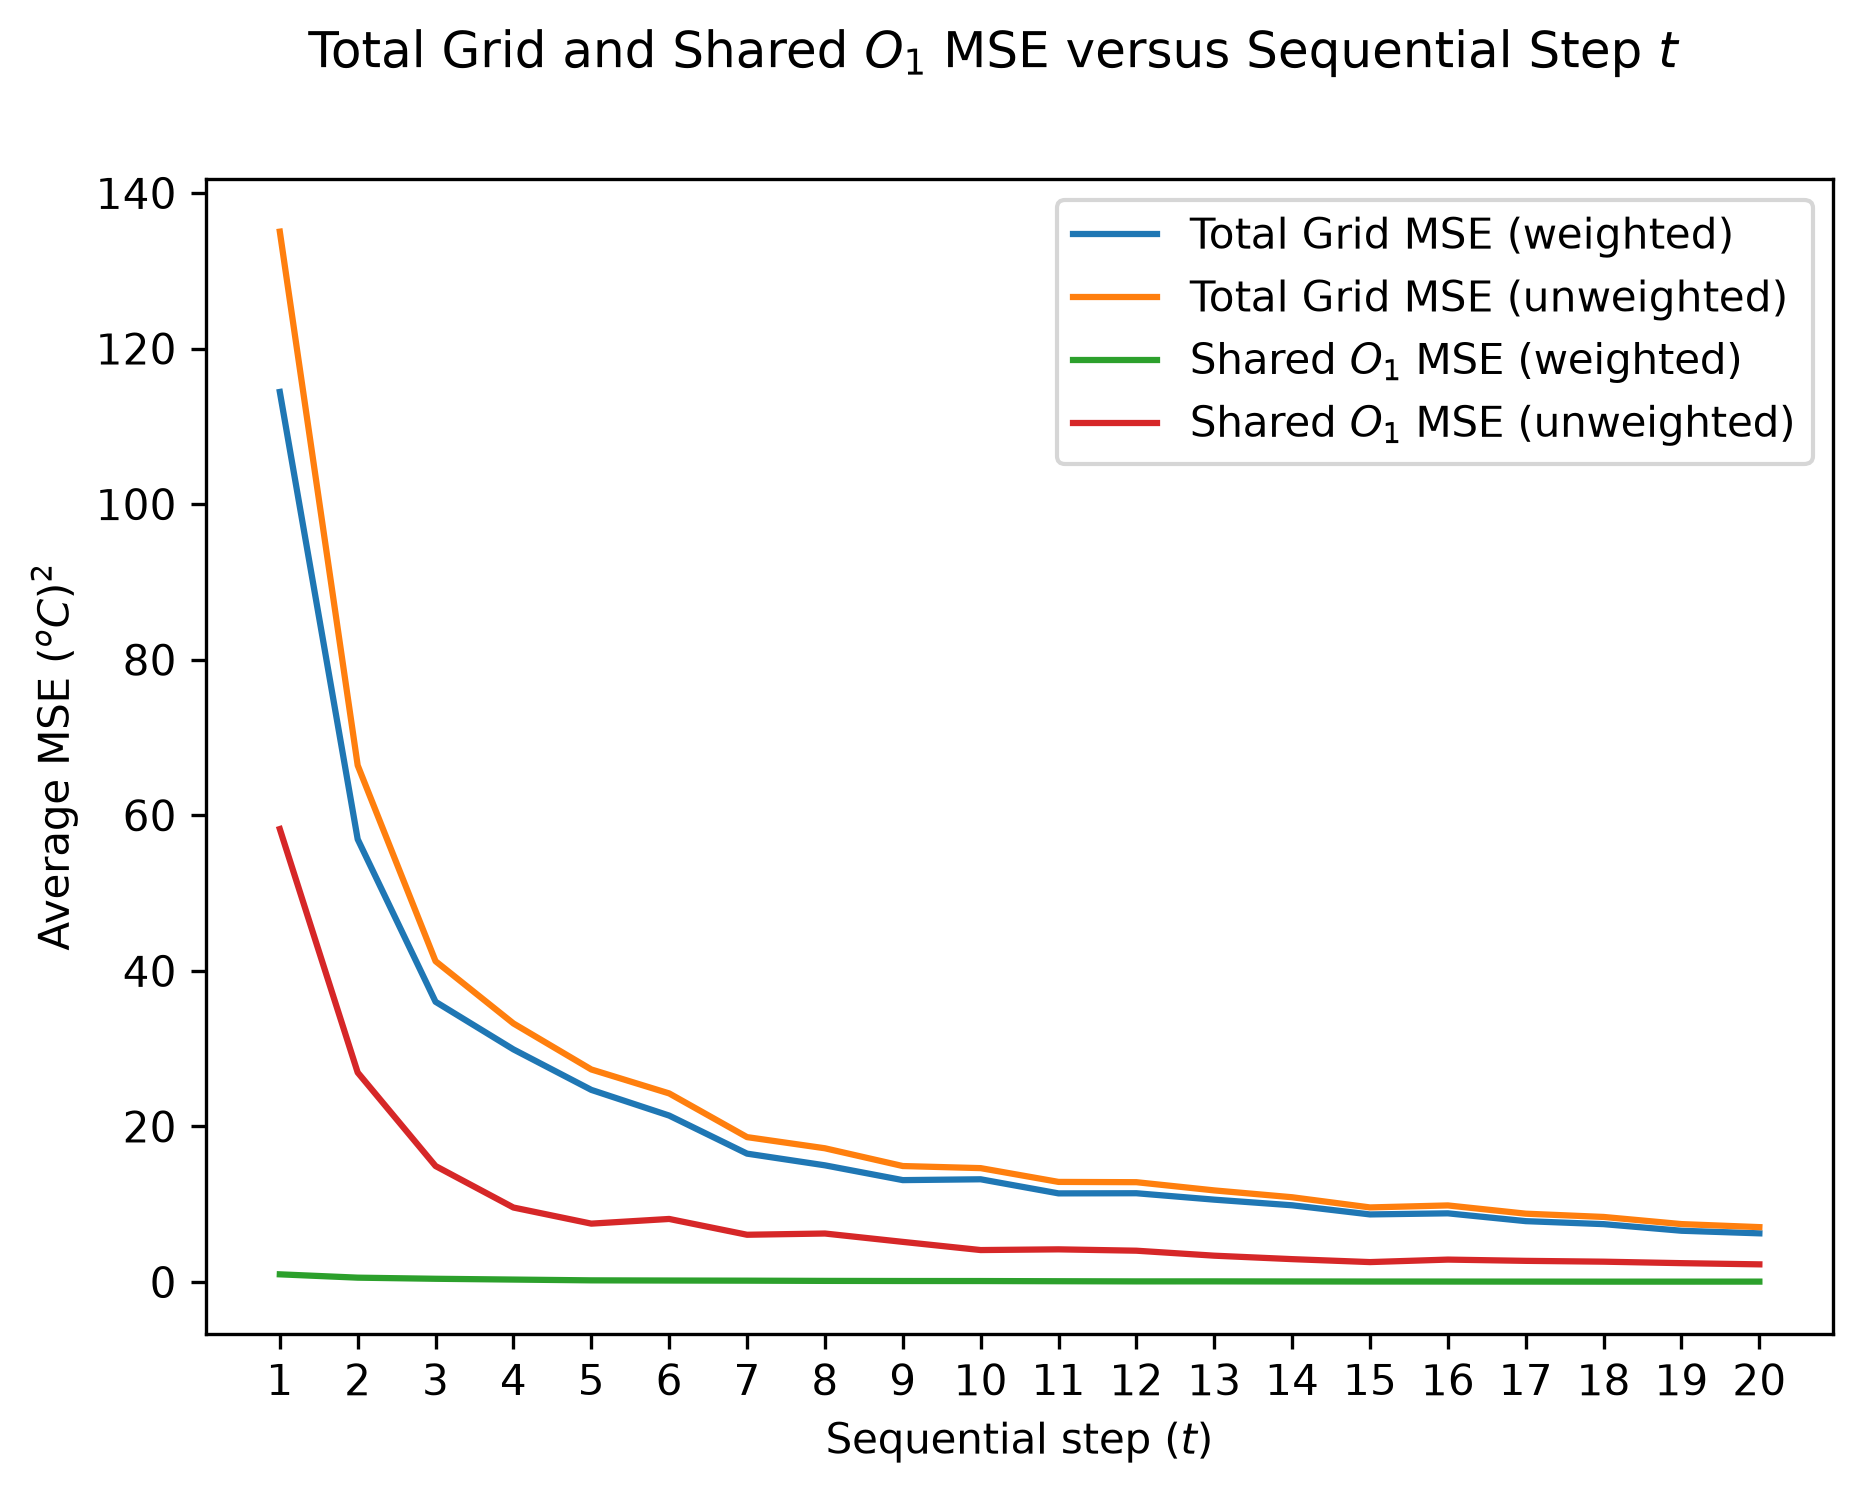
\includegraphics[width=0.5\textwidth]{Figures/mse_plot.png}
    \captionsetup{justification=centering}
    \caption{Plot of MSE versus $t$ for both weighted and unweighted sensor fusion for both the total grid and for $\mathcal O_1$.}
    \label{fig:mse_plot}
\end{figure}

To visualize the convergence of the grid to the true measurement, Figure \ref{fig:temperature_seq} shows the initial fused measurements at $t=1$ and the final fused measurements at $t=20$ for both the weighted and unweighted fusion. As seen, in both the weighted and unweighted sensor fusions, the final temperature estimates are nearly identical to the true temperatures from Figure \ref{fig:true_temperature_graph_network}, as reflected by the decreasing MSE through $t$ in Figure \ref{fig:mse_plot}. The difference is in the \textit{initial} grid estimate, where the weighted fusion already had a good estimate of $\mathcal V^{(1)}$ while the unweighted estimate was uncertain due to the naive fusion of uncertain measurements with the measurement of robot 1. What this Figure shows, however, is that even in the case that robots \textit{do not} know the uncertainty of their own measurements, or in the case that the uncertainty of their own measurements are changing, simply applying \textit{repeated} measurements and fusing them in an unweighted way will still converge to the true value, providing a minimalist approach to estimation.

\begin{figure}[htb]
    \centering
    \begin{subfigure}[t]{0.4\textwidth}
        \centering
        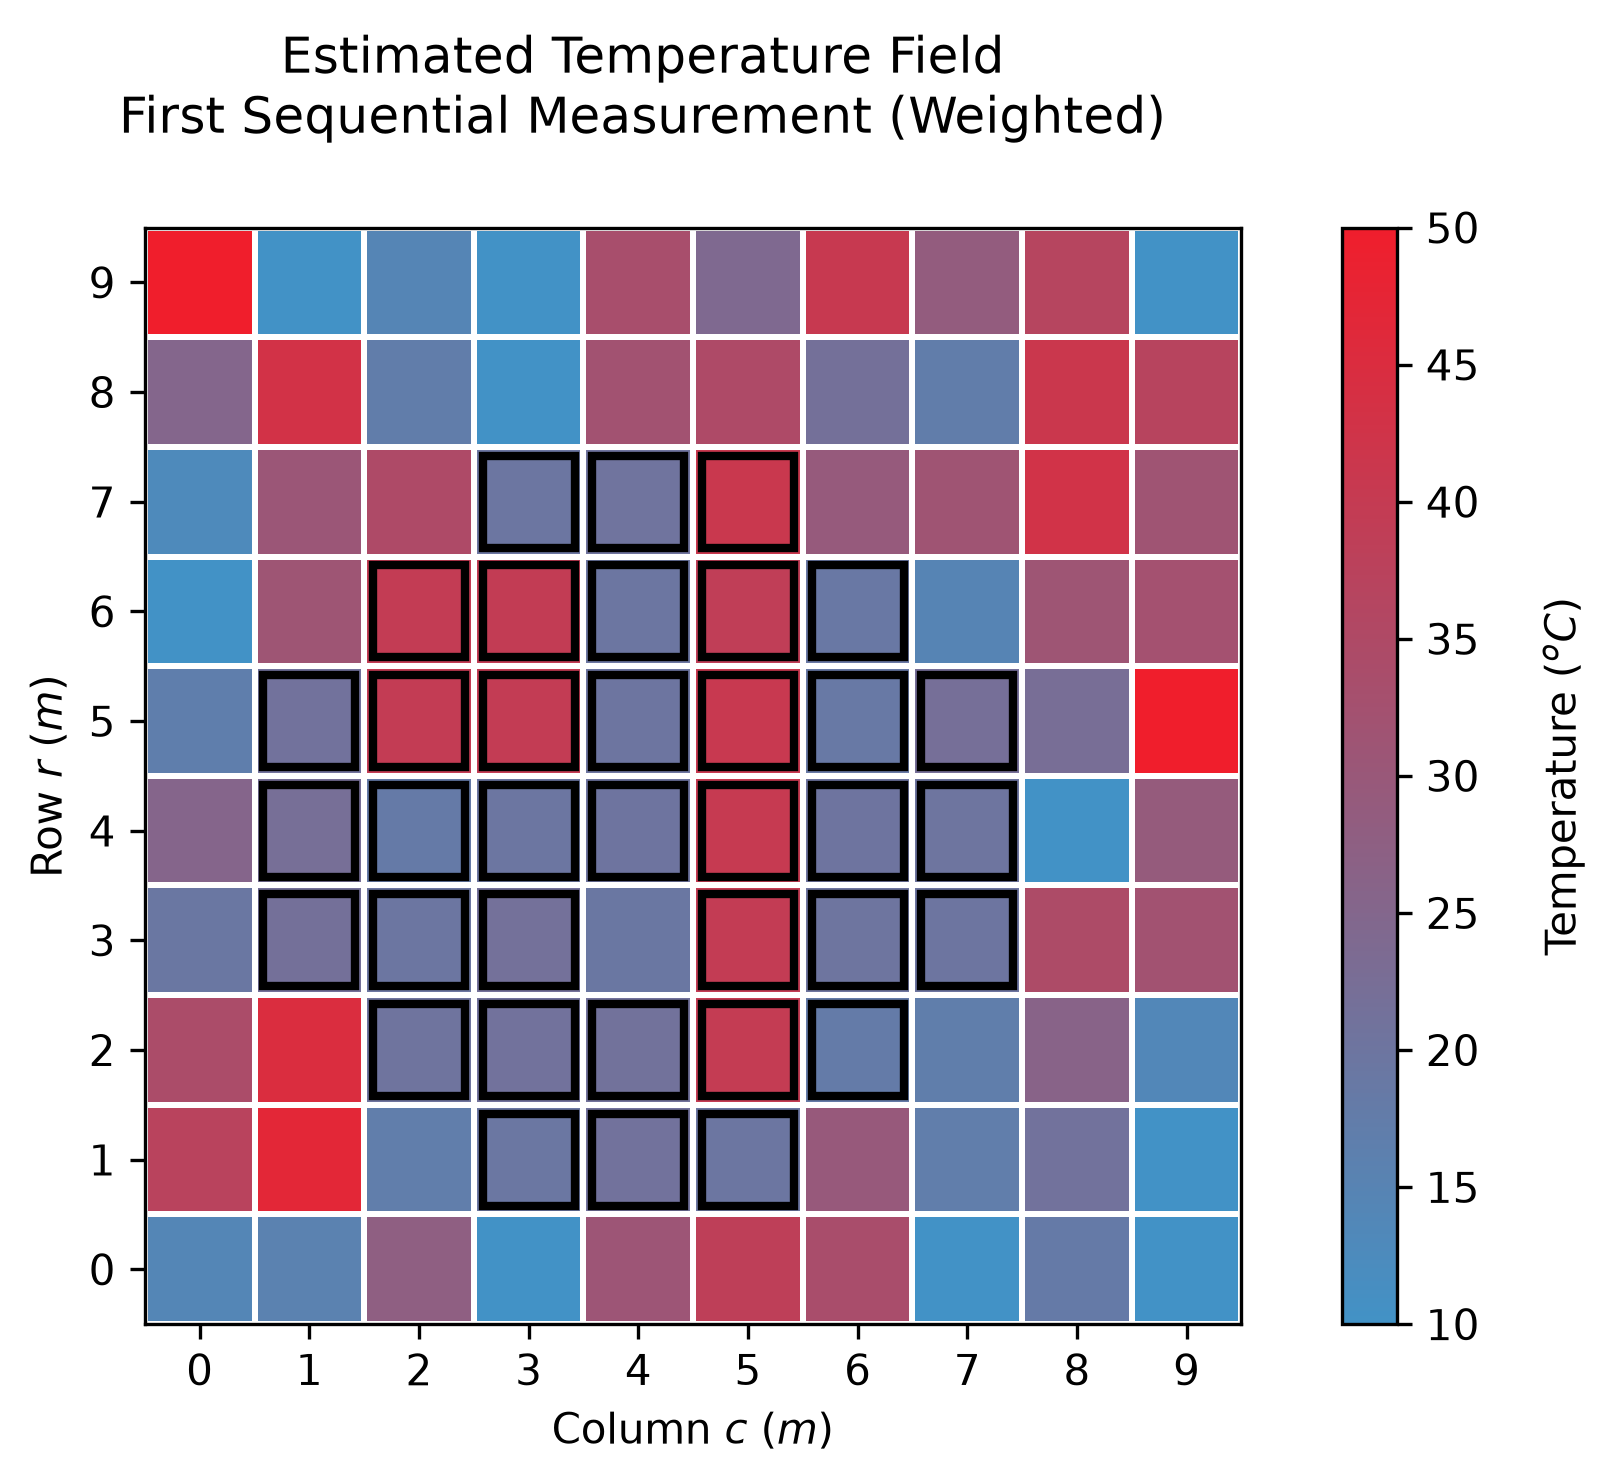
\includegraphics[width=\textwidth]{Figures/temperature_w_0_6.png}
        \captionsetup{justification=centering}
        \caption{Initial temperature field estimate for weighted sensor fusion.}
        % \label{fig:}
    \end{subfigure}\hfill
    \begin{subfigure}[t]{0.4\textwidth}
        \centering
        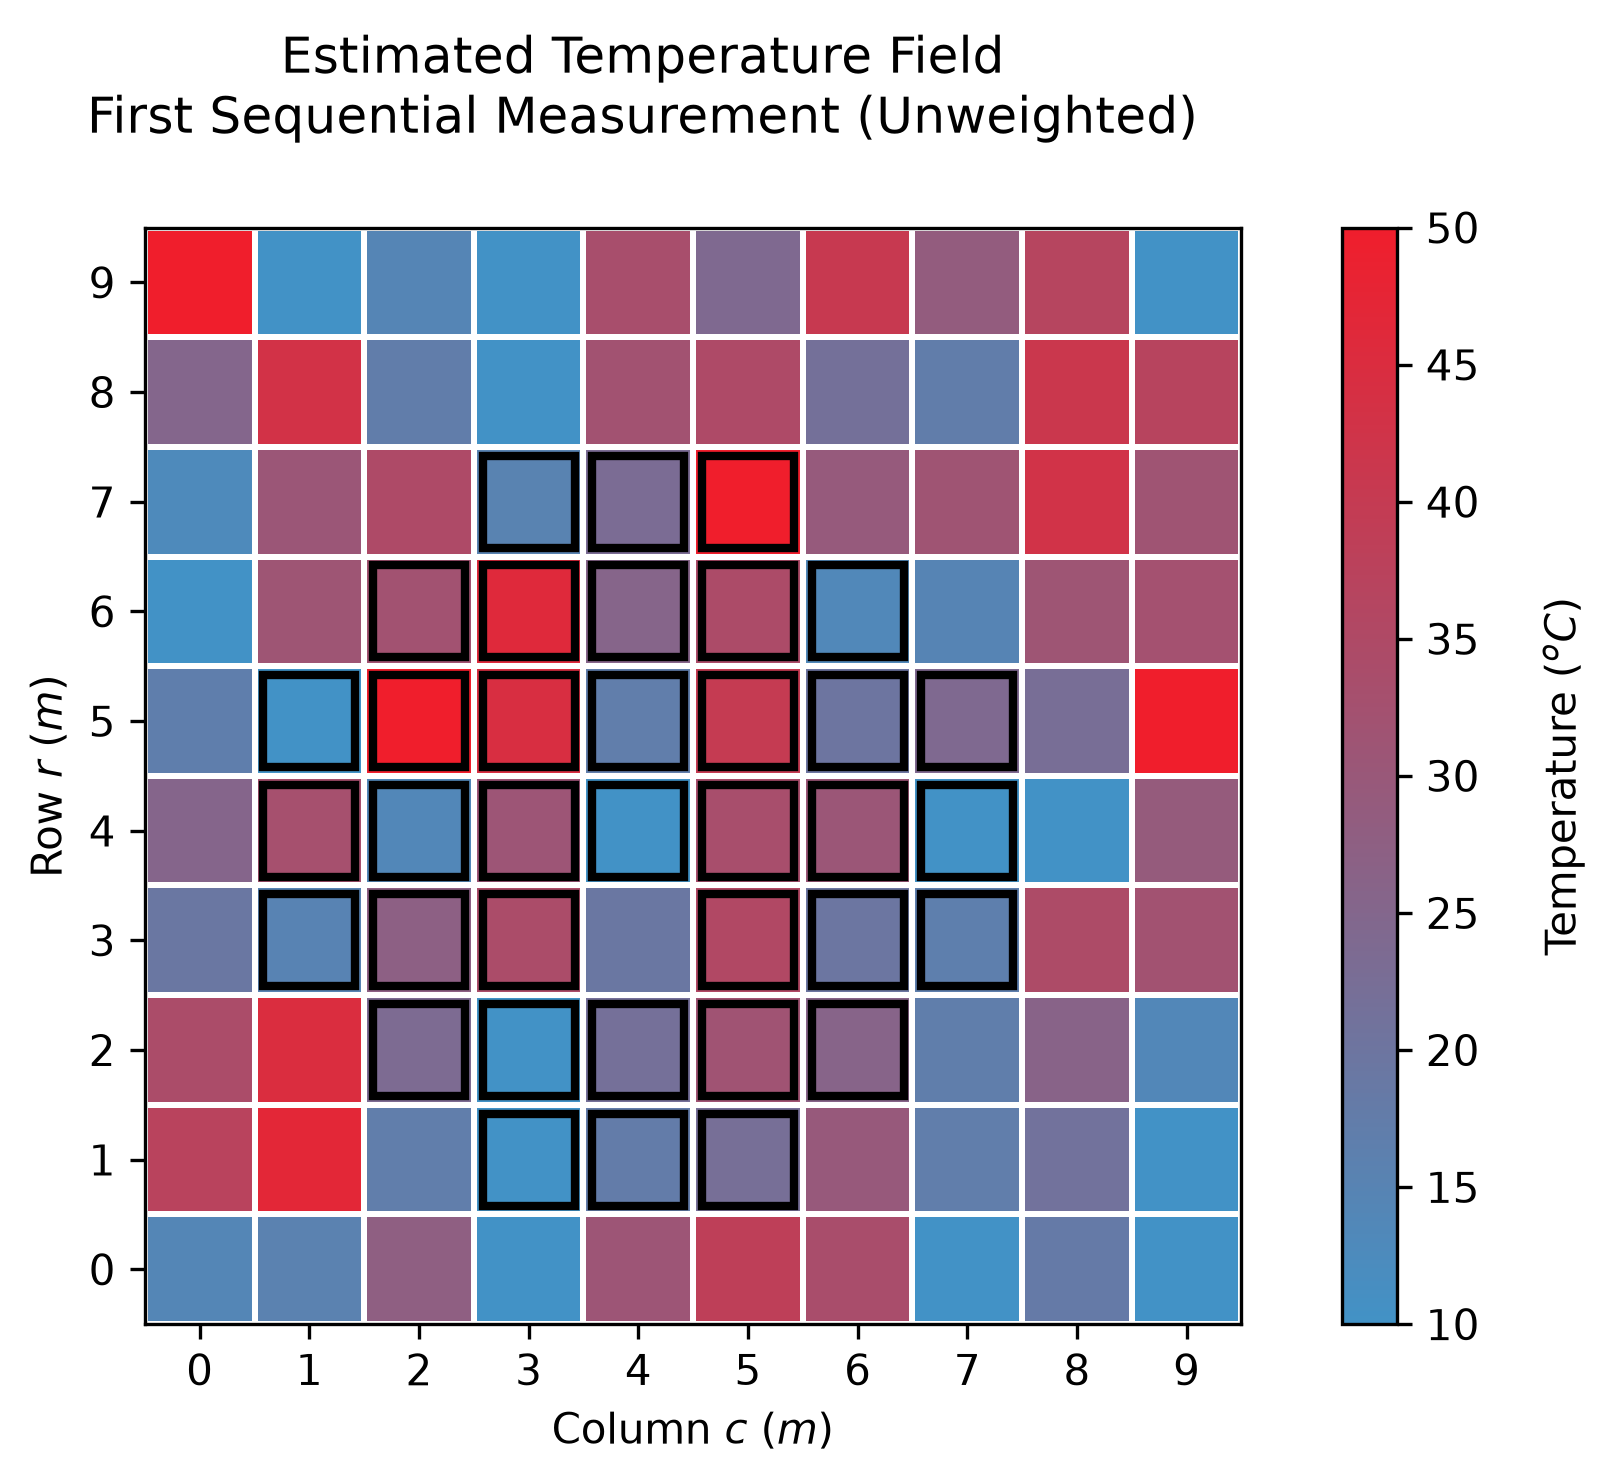
\includegraphics[width=\textwidth]{Figures/temperature_u_0_6.png}
        \captionsetup{justification=centering}
        \caption{Initial temperature field estimate for unweighted sensor fusion.}
        % \label{fig:}
    \end{subfigure}\\
    \begin{subfigure}[t]{0.4\textwidth}
        \centering
        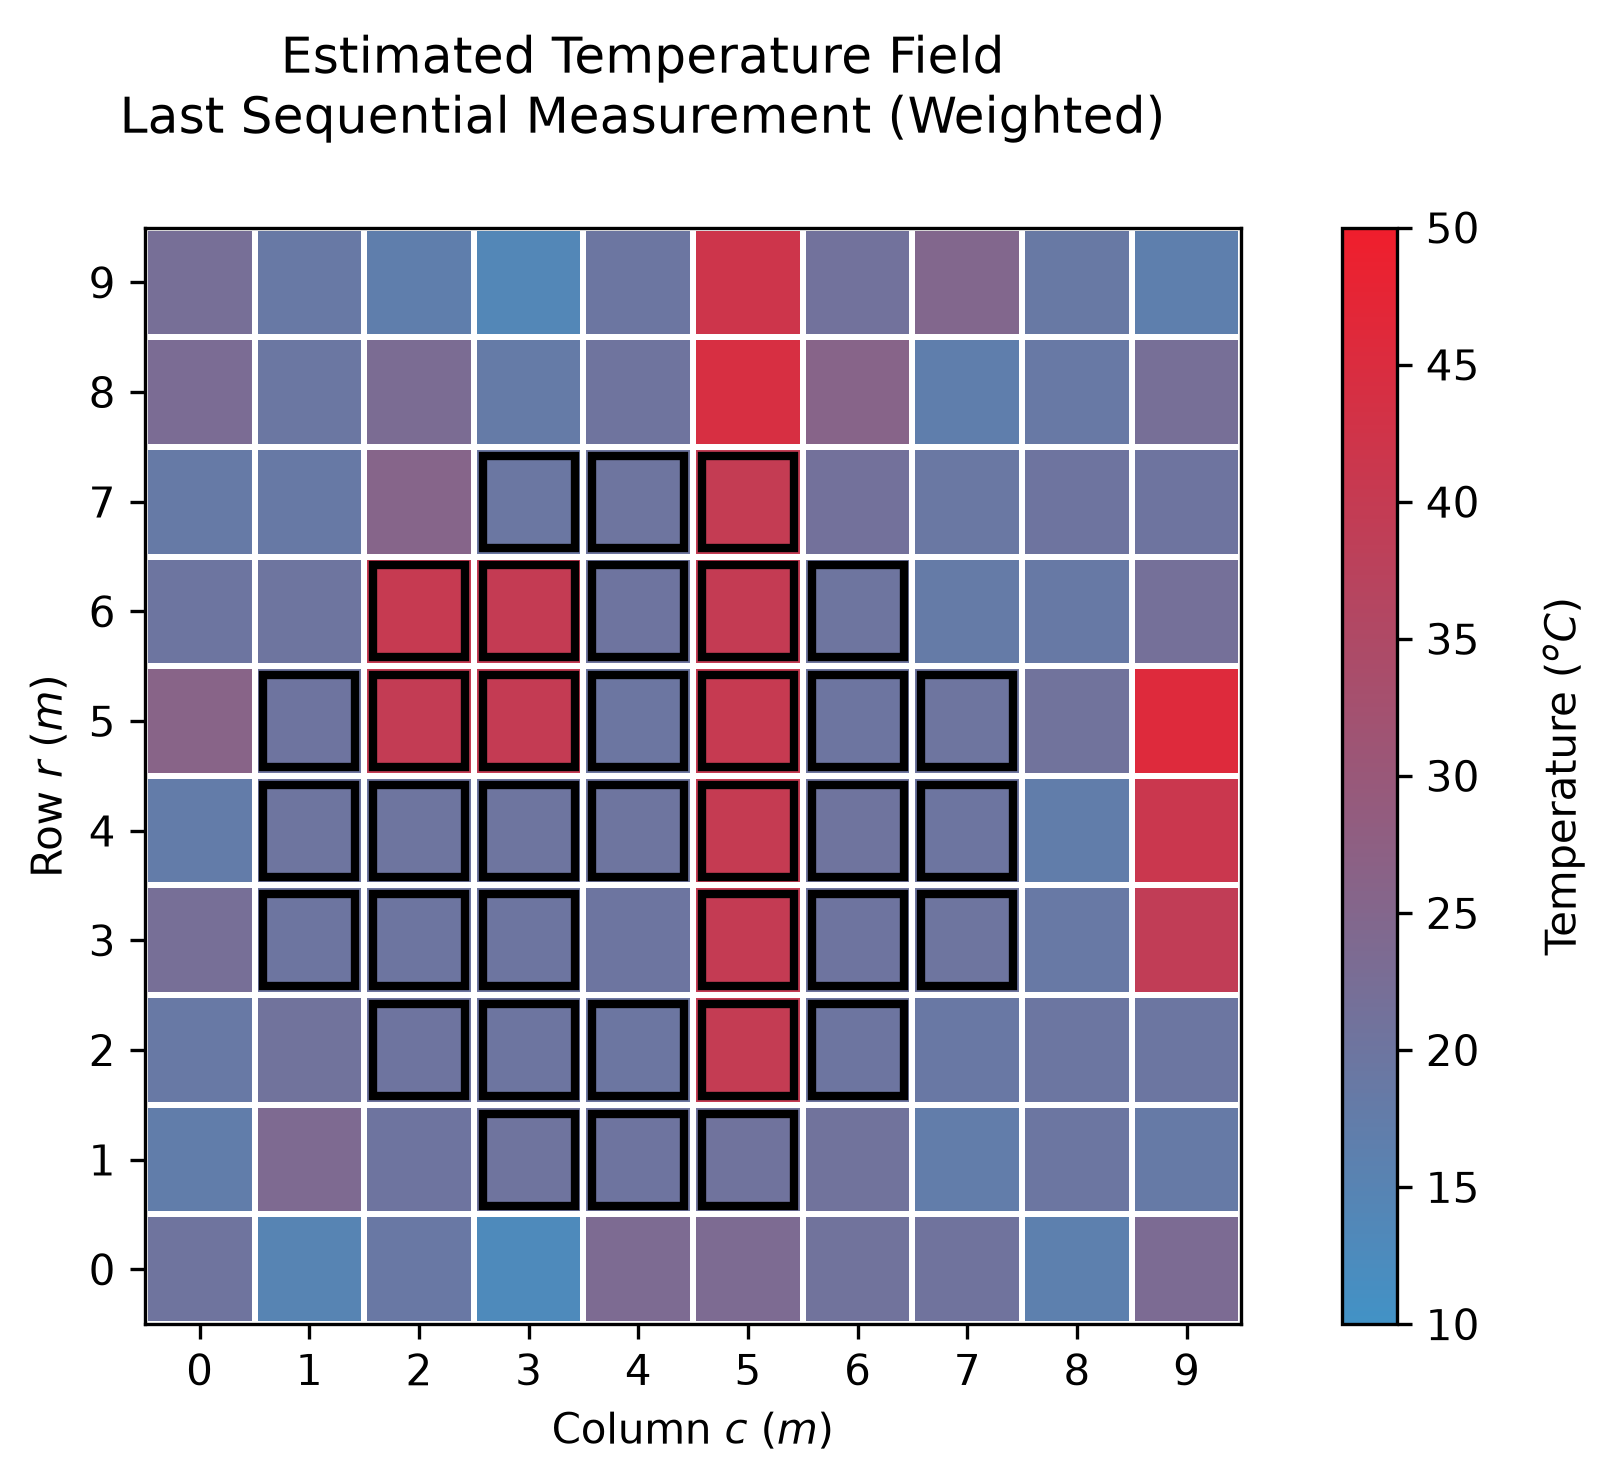
\includegraphics[width=\textwidth]{Figures/temperature_w_f_6.png}
        \captionsetup{justification=centering}
        \caption{Final temperature field estimate for weighted sensor fusion.}
        % \label{fig:}
    \end{subfigure}\hfill
    \begin{subfigure}[t]{0.4\textwidth}
        \centering
        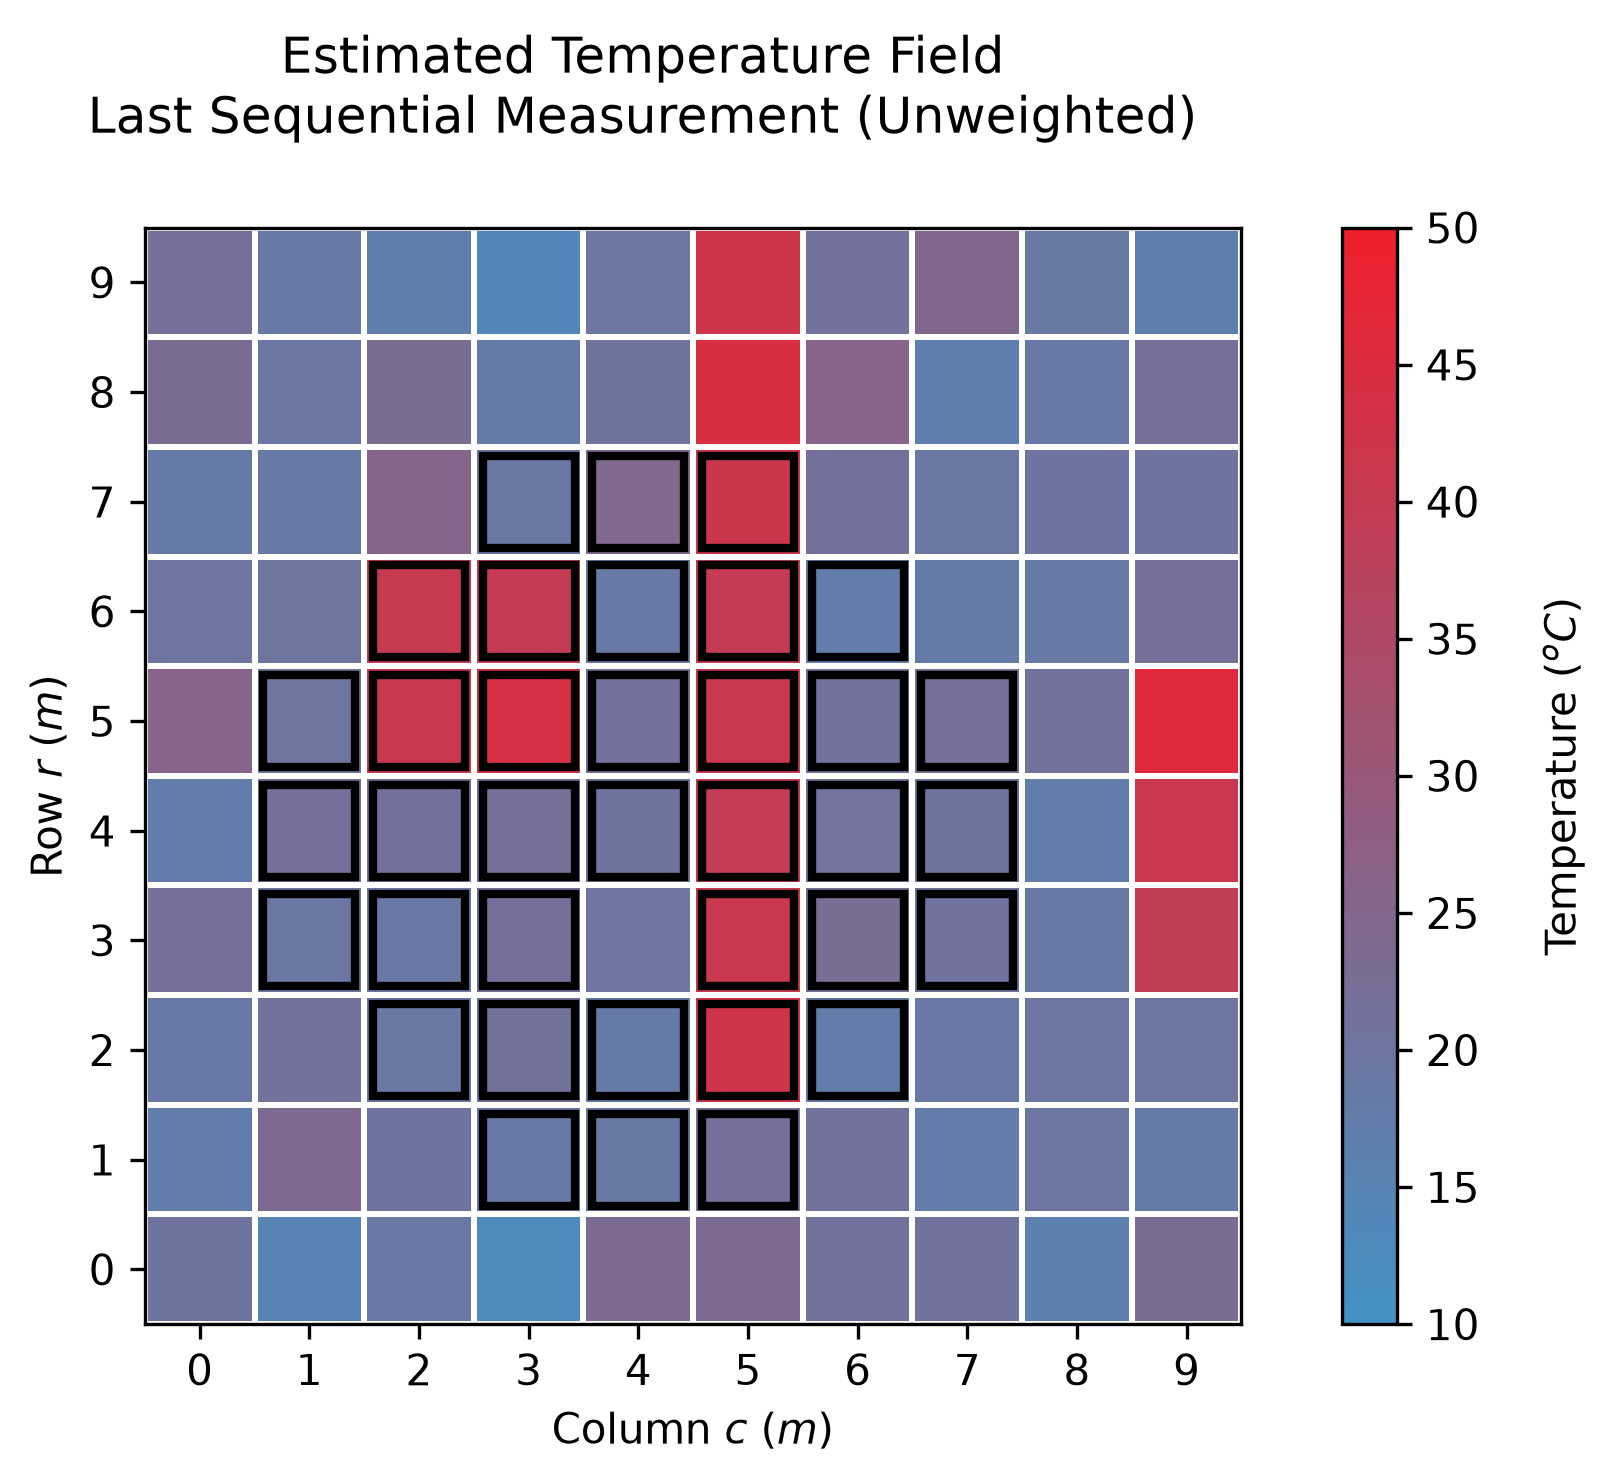
\includegraphics[width=\textwidth]{Figures/temperature_u_f_6.png}
        \captionsetup{justification=centering}
        \caption{Final temperature field estimate for unweighted sensor fusion.}
        % \label{fig:}
    \end{subfigure}
    \captionsetup{justification=centering}
    \caption{Cells within $\mathcal O_1$ are bolded in a \textbf{black} square.}
    \label{fig:temperature_seq}
\end{figure}


%%%%% REFERENCES
% \clearpage
% \printbibliography[title={\textbf{REFERENCES}}]

%%%% APPENDIX
% \appendix\appendixpagenumbering
% \section{}\label{app:}

\end{document}
